% Created by tikzDevice version 0.7.0 on 2014-07-29 12:04:59
% !TEX encoding = UTF-8 Unicode
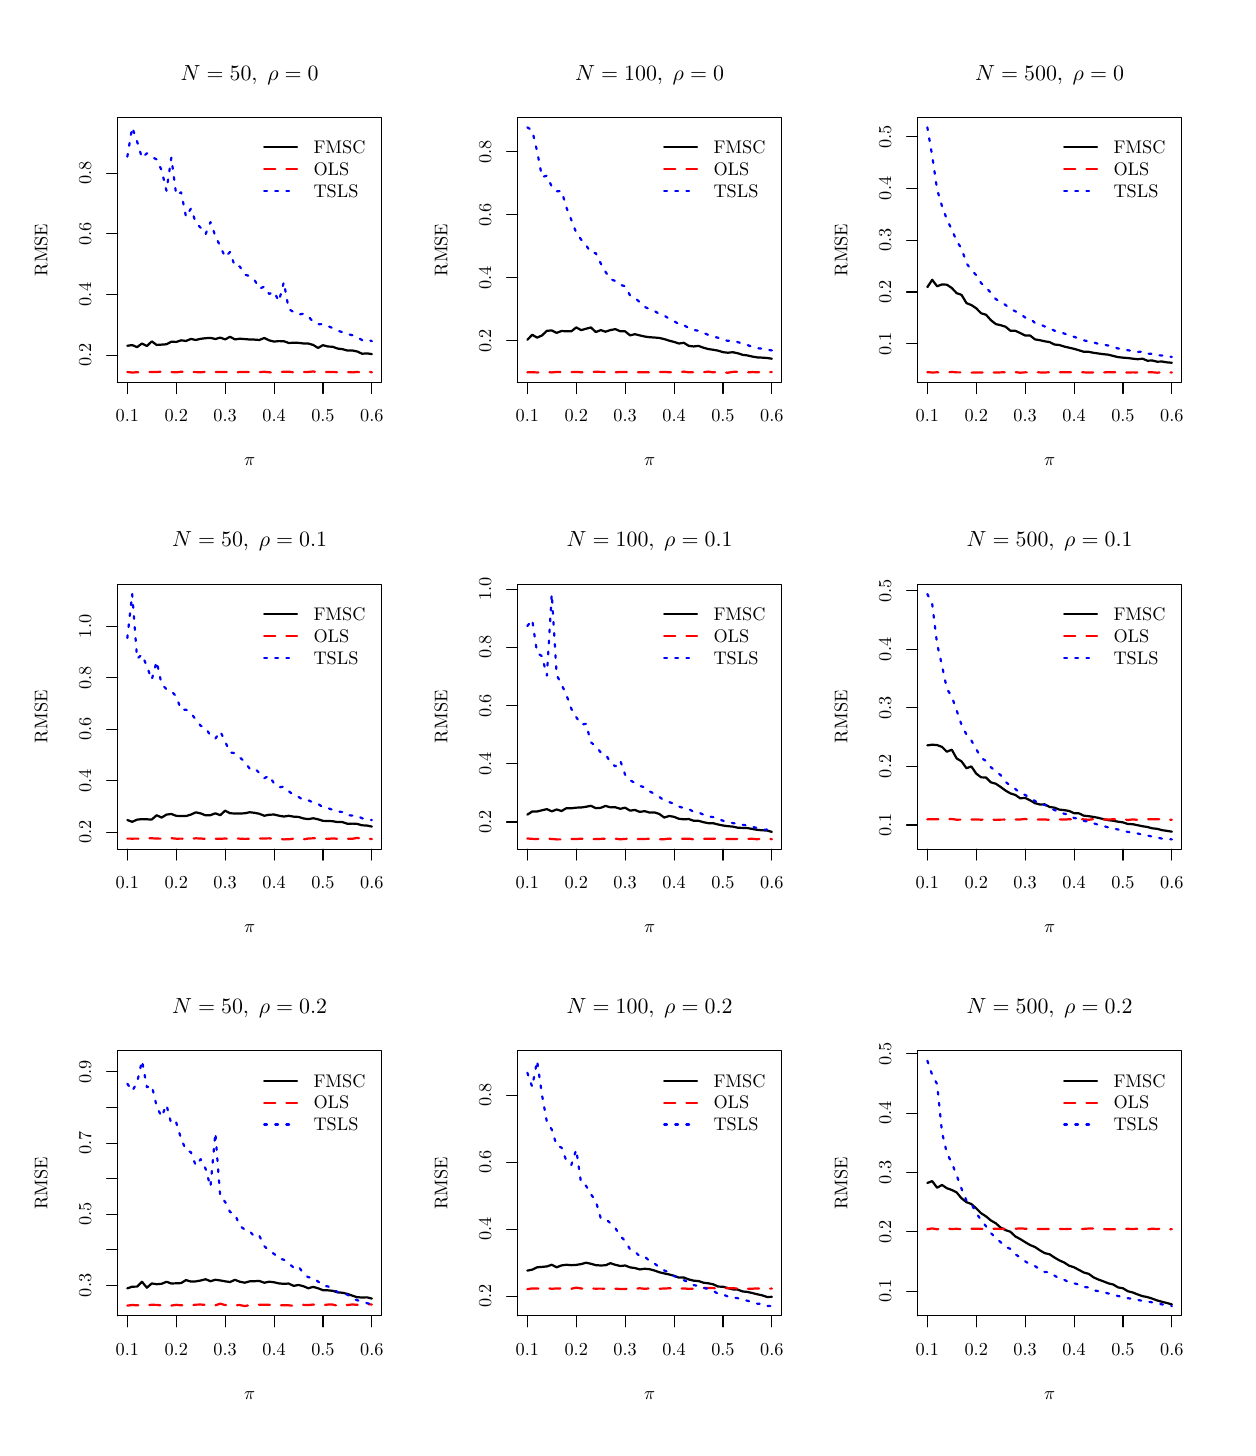
\begin{tikzpicture}[x=1pt,y=1pt]
\definecolor[named]{fillColor}{rgb}{1.00,1.00,1.00}
\path[use as bounding box,fill=fillColor,fill opacity=0.00] (0,0) rectangle (433.62,505.89);
\begin{scope}
\path[clip] ( 32.47,377.65) rectangle (127.91,473.42);
\definecolor[named]{drawColor}{rgb}{0.00,0.00,0.00}

\path[draw=drawColor,line width= 0.8pt,line join=round,line cap=round] ( 36.01,390.94) --
	( 37.77,391.19) --
	( 39.54,390.45) --
	( 41.31,391.76) --
	( 43.08,390.85) --
	( 44.84,392.53) --
	( 46.61,391.24) --
	( 48.38,391.36) --
	( 50.15,391.48) --
	( 51.91,392.41) --
	( 53.68,392.33) --
	( 55.45,392.91) --
	( 57.21,392.68) --
	( 58.98,393.41) --
	( 60.75,393.04) --
	( 62.52,393.46) --
	( 64.28,393.67) --
	( 66.05,393.80) --
	( 67.82,393.38) --
	( 69.59,393.90) --
	( 71.35,393.23) --
	( 73.12,394.20) --
	( 74.89,393.24) --
	( 76.66,393.49) --
	( 78.42,393.36) --
	( 80.19,393.21) --
	( 81.96,393.17) --
	( 83.72,393.03) --
	( 85.49,393.75) --
	( 87.26,392.90) --
	( 89.03,392.46) --
	( 90.79,392.62) --
	( 92.56,392.59) --
	( 94.33,391.96) --
	( 96.10,392.03) --
	( 97.86,391.99) --
	( 99.63,391.78) --
	(101.40,391.74) --
	(103.17,391.24) --
	(104.93,390.16) --
	(106.70,391.15) --
	(108.47,390.67) --
	(110.23,390.58) --
	(112.00,389.93) --
	(113.77,389.71) --
	(115.54,389.21) --
	(117.30,389.24) --
	(119.07,388.88) --
	(120.84,388.06) --
	(122.61,388.19) --
	(124.37,387.93);
\end{scope}
\begin{scope}
\path[clip] (  0.00,  0.00) rectangle (433.62,505.89);
\definecolor[named]{drawColor}{rgb}{0.00,0.00,0.00}

\path[draw=drawColor,line width= 0.4pt,line join=round,line cap=round] ( 36.01,377.65) -- (124.37,377.65);

\path[draw=drawColor,line width= 0.4pt,line join=round,line cap=round] ( 36.01,377.65) -- ( 36.01,373.69);

\path[draw=drawColor,line width= 0.4pt,line join=round,line cap=round] ( 53.68,377.65) -- ( 53.68,373.69);

\path[draw=drawColor,line width= 0.4pt,line join=round,line cap=round] ( 71.35,377.65) -- ( 71.35,373.69);

\path[draw=drawColor,line width= 0.4pt,line join=round,line cap=round] ( 89.03,377.65) -- ( 89.03,373.69);

\path[draw=drawColor,line width= 0.4pt,line join=round,line cap=round] (106.70,377.65) -- (106.70,373.69);

\path[draw=drawColor,line width= 0.4pt,line join=round,line cap=round] (124.37,377.65) -- (124.37,373.69);

\node[text=drawColor,anchor=base,inner sep=0pt, outer sep=0pt, scale=  0.66] at ( 36.01,363.40) {0.1};

\node[text=drawColor,anchor=base,inner sep=0pt, outer sep=0pt, scale=  0.66] at ( 53.68,363.40) {0.2};

\node[text=drawColor,anchor=base,inner sep=0pt, outer sep=0pt, scale=  0.66] at ( 71.35,363.40) {0.3};

\node[text=drawColor,anchor=base,inner sep=0pt, outer sep=0pt, scale=  0.66] at ( 89.03,363.40) {0.4};

\node[text=drawColor,anchor=base,inner sep=0pt, outer sep=0pt, scale=  0.66] at (106.70,363.40) {0.5};

\node[text=drawColor,anchor=base,inner sep=0pt, outer sep=0pt, scale=  0.66] at (124.37,363.40) {0.6};

\path[draw=drawColor,line width= 0.4pt,line join=round,line cap=round] ( 32.47,387.54) -- ( 32.47,453.30);

\path[draw=drawColor,line width= 0.4pt,line join=round,line cap=round] ( 32.47,387.54) -- ( 28.51,387.54);

\path[draw=drawColor,line width= 0.4pt,line join=round,line cap=round] ( 32.47,409.46) -- ( 28.51,409.46);

\path[draw=drawColor,line width= 0.4pt,line join=round,line cap=round] ( 32.47,431.38) -- ( 28.51,431.38);

\path[draw=drawColor,line width= 0.4pt,line join=round,line cap=round] ( 32.47,453.30) -- ( 28.51,453.30);

\node[text=drawColor,rotate= 90.00,anchor=base,inner sep=0pt, outer sep=0pt, scale=  0.66] at ( 22.97,387.54) {0.2};

\node[text=drawColor,rotate= 90.00,anchor=base,inner sep=0pt, outer sep=0pt, scale=  0.66] at ( 22.97,409.46) {0.4};

\node[text=drawColor,rotate= 90.00,anchor=base,inner sep=0pt, outer sep=0pt, scale=  0.66] at ( 22.97,431.38) {0.6};

\node[text=drawColor,rotate= 90.00,anchor=base,inner sep=0pt, outer sep=0pt, scale=  0.66] at ( 22.97,453.30) {0.8};

\path[draw=drawColor,line width= 0.4pt,line join=round,line cap=round] ( 32.47,377.65) --
	(127.91,377.65) --
	(127.91,473.42) --
	( 32.47,473.42) --
	( 32.47,377.65);
\end{scope}
\begin{scope}
\path[clip] (  0.00,337.26) rectangle (144.54,505.89);
\definecolor[named]{drawColor}{rgb}{0.00,0.00,0.00}

\node[text=drawColor,anchor=base,inner sep=0pt, outer sep=0pt, scale=  0.79] at ( 80.19,486.92) {\bfseries $N=50, \;\rho=0$};

\node[text=drawColor,anchor=base,inner sep=0pt, outer sep=0pt, scale=  0.66] at ( 80.19,347.56) {$\pi$};

\node[text=drawColor,rotate= 90.00,anchor=base,inner sep=0pt, outer sep=0pt, scale=  0.66] at (  7.13,425.53) {RMSE};
\end{scope}
\begin{scope}
\path[clip] ( 32.47,377.65) rectangle (127.91,473.42);
\definecolor[named]{drawColor}{rgb}{1.00,0.00,0.00}

\path[draw=drawColor,line width= 0.8pt,dash pattern=on 4pt off 4pt ,line join=round,line cap=round] ( 36.01,381.46) --
	( 37.77,381.27) --
	( 39.54,381.38) --
	( 41.31,381.37) --
	( 43.08,381.49) --
	( 44.84,381.46) --
	( 46.61,381.47) --
	( 48.38,381.58) --
	( 50.15,381.41) --
	( 51.91,381.43) --
	( 53.68,381.34) --
	( 55.45,381.55) --
	( 57.21,381.46) --
	( 58.98,381.48) --
	( 60.75,381.42) --
	( 62.52,381.36) --
	( 64.28,381.55) --
	( 66.05,381.46) --
	( 67.82,381.43) --
	( 69.59,381.46) --
	( 71.35,381.47) --
	( 73.12,381.41) --
	( 74.89,381.20) --
	( 76.66,381.47) --
	( 78.42,381.49) --
	( 80.19,381.43) --
	( 81.96,381.23) --
	( 83.72,381.41) --
	( 85.49,381.55) --
	( 87.26,381.36) --
	( 89.03,381.22) --
	( 90.79,381.34) --
	( 92.56,381.59) --
	( 94.33,381.59) --
	( 96.10,381.35) --
	( 97.86,381.39) --
	( 99.63,381.45) --
	(101.40,381.49) --
	(103.17,381.66) --
	(104.93,381.31) --
	(106.70,381.52) --
	(108.47,381.45) --
	(110.23,381.44) --
	(112.00,381.39) --
	(113.77,381.43) --
	(115.54,381.45) --
	(117.30,381.32) --
	(119.07,381.48) --
	(120.84,381.28) --
	(122.61,381.67) --
	(124.37,381.36);
\definecolor[named]{drawColor}{rgb}{0.00,0.00,1.00}

\path[draw=drawColor,line width= 0.8pt,dash pattern=on 1pt off 3pt ,line join=round,line cap=round] ( 36.01,459.27) --
	( 37.77,469.87) --
	( 39.54,464.75) --
	( 41.31,458.79) --
	( 43.08,460.51) --
	( 44.84,459.16) --
	( 46.61,458.27) --
	( 48.38,454.40) --
	( 50.15,446.99) --
	( 51.91,458.89) --
	( 53.68,445.44) --
	( 55.45,446.39) --
	( 57.21,437.53) --
	( 58.98,440.52) --
	( 60.75,435.49) --
	( 62.52,433.55) --
	( 64.28,431.23) --
	( 66.05,435.62) --
	( 67.82,430.58) --
	( 69.59,426.86) --
	( 71.35,422.97) --
	( 73.12,424.82) --
	( 74.89,419.58) --
	( 76.66,419.59) --
	( 78.42,416.67) --
	( 80.19,416.13) --
	( 81.96,414.74) --
	( 83.72,411.58) --
	( 85.49,412.29) --
	( 87.26,409.67) --
	( 89.03,410.48) --
	( 90.79,406.99) --
	( 92.56,413.94) --
	( 94.33,404.18) --
	( 96.10,403.14) --
	( 97.86,402.21) --
	( 99.63,402.52) --
	(101.40,401.55) --
	(103.17,399.59) --
	(104.93,398.75) --
	(106.70,398.76) --
	(108.47,398.06) --
	(110.23,397.33) --
	(112.00,396.38) --
	(113.77,395.86) --
	(115.54,395.23) --
	(117.30,394.74) --
	(119.07,394.09) --
	(120.84,392.99) --
	(122.61,393.25) --
	(124.37,392.61);
\definecolor[named]{drawColor}{rgb}{0.00,0.00,0.00}

\path[draw=drawColor,line width= 0.8pt,line join=round,line cap=round] ( 85.47,462.63) -- ( 97.35,462.63);
\definecolor[named]{drawColor}{rgb}{1.00,0.00,0.00}

\path[draw=drawColor,line width= 0.8pt,dash pattern=on 4pt off 4pt ,line join=round,line cap=round] ( 85.47,454.71) -- ( 97.35,454.71);
\definecolor[named]{drawColor}{rgb}{0.00,0.00,1.00}

\path[draw=drawColor,line width= 0.8pt,dash pattern=on 1pt off 3pt ,line join=round,line cap=round] ( 85.47,446.79) -- ( 97.35,446.79);
\definecolor[named]{drawColor}{rgb}{0.00,0.00,0.00}

\node[text=drawColor,anchor=base west,inner sep=0pt, outer sep=0pt, scale=  0.66] at (103.29,460.35) {FMSC};

\node[text=drawColor,anchor=base west,inner sep=0pt, outer sep=0pt, scale=  0.66] at (103.29,452.43) {OLS};

\node[text=drawColor,anchor=base west,inner sep=0pt, outer sep=0pt, scale=  0.66] at (103.29,444.51) {TSLS};
\end{scope}
\begin{scope}
\path[clip] (177.01,377.65) rectangle (272.45,473.42);
\definecolor[named]{drawColor}{rgb}{0.00,0.00,0.00}

\path[draw=drawColor,line width= 0.8pt,line join=round,line cap=round] (180.55,393.08) --
	(182.31,394.92) --
	(184.08,393.88) --
	(185.85,394.67) --
	(187.62,396.35) --
	(189.38,396.48) --
	(191.15,395.61) --
	(192.92,396.28) --
	(194.69,396.17) --
	(196.45,396.15) --
	(198.22,397.58) --
	(199.99,396.59) --
	(201.75,397.08) --
	(203.52,397.56) --
	(205.29,395.90) --
	(207.06,396.59) --
	(208.82,396.02) --
	(210.59,396.62) --
	(212.36,396.94) --
	(214.13,396.19) --
	(215.89,396.15) --
	(217.66,394.70) --
	(219.43,395.12) --
	(221.20,394.68) --
	(222.96,394.28) --
	(224.73,394.03) --
	(226.50,393.92) --
	(228.26,393.76) --
	(230.03,393.35) --
	(231.80,392.79) --
	(233.57,392.33) --
	(235.33,391.75) --
	(237.10,392.02) --
	(238.87,390.91) --
	(240.64,390.69) --
	(242.40,390.90) --
	(244.17,390.25) --
	(245.94,389.75) --
	(247.71,389.50) --
	(249.47,389.18) --
	(251.24,388.63) --
	(253.01,388.43) --
	(254.77,388.61) --
	(256.54,388.25) --
	(258.31,387.67) --
	(260.08,387.45) --
	(261.84,387.04) --
	(263.61,386.74) --
	(265.38,386.65) --
	(267.15,386.53) --
	(268.91,386.26);
\end{scope}
\begin{scope}
\path[clip] (  0.00,  0.00) rectangle (433.62,505.89);
\definecolor[named]{drawColor}{rgb}{0.00,0.00,0.00}

\path[draw=drawColor,line width= 0.4pt,line join=round,line cap=round] (180.55,377.65) -- (268.91,377.65);

\path[draw=drawColor,line width= 0.4pt,line join=round,line cap=round] (180.55,377.65) -- (180.55,373.69);

\path[draw=drawColor,line width= 0.4pt,line join=round,line cap=round] (198.22,377.65) -- (198.22,373.69);

\path[draw=drawColor,line width= 0.4pt,line join=round,line cap=round] (215.89,377.65) -- (215.89,373.69);

\path[draw=drawColor,line width= 0.4pt,line join=round,line cap=round] (233.57,377.65) -- (233.57,373.69);

\path[draw=drawColor,line width= 0.4pt,line join=round,line cap=round] (251.24,377.65) -- (251.24,373.69);

\path[draw=drawColor,line width= 0.4pt,line join=round,line cap=round] (268.91,377.65) -- (268.91,373.69);

\node[text=drawColor,anchor=base,inner sep=0pt, outer sep=0pt, scale=  0.66] at (180.55,363.40) {0.1};

\node[text=drawColor,anchor=base,inner sep=0pt, outer sep=0pt, scale=  0.66] at (198.22,363.40) {0.2};

\node[text=drawColor,anchor=base,inner sep=0pt, outer sep=0pt, scale=  0.66] at (215.89,363.40) {0.3};

\node[text=drawColor,anchor=base,inner sep=0pt, outer sep=0pt, scale=  0.66] at (233.57,363.40) {0.4};

\node[text=drawColor,anchor=base,inner sep=0pt, outer sep=0pt, scale=  0.66] at (251.24,363.40) {0.5};

\node[text=drawColor,anchor=base,inner sep=0pt, outer sep=0pt, scale=  0.66] at (268.91,363.40) {0.6};

\path[draw=drawColor,line width= 0.4pt,line join=round,line cap=round] (177.01,392.72) -- (177.01,461.10);

\path[draw=drawColor,line width= 0.4pt,line join=round,line cap=round] (177.01,392.72) -- (173.05,392.72);

\path[draw=drawColor,line width= 0.4pt,line join=round,line cap=round] (177.01,415.51) -- (173.05,415.51);

\path[draw=drawColor,line width= 0.4pt,line join=round,line cap=round] (177.01,438.31) -- (173.05,438.31);

\path[draw=drawColor,line width= 0.4pt,line join=round,line cap=round] (177.01,461.10) -- (173.05,461.10);

\node[text=drawColor,rotate= 90.00,anchor=base,inner sep=0pt, outer sep=0pt, scale=  0.66] at (167.51,392.72) {0.2};

\node[text=drawColor,rotate= 90.00,anchor=base,inner sep=0pt, outer sep=0pt, scale=  0.66] at (167.51,415.51) {0.4};

\node[text=drawColor,rotate= 90.00,anchor=base,inner sep=0pt, outer sep=0pt, scale=  0.66] at (167.51,438.31) {0.6};

\node[text=drawColor,rotate= 90.00,anchor=base,inner sep=0pt, outer sep=0pt, scale=  0.66] at (167.51,461.10) {0.8};

\path[draw=drawColor,line width= 0.4pt,line join=round,line cap=round] (177.01,377.65) --
	(272.45,377.65) --
	(272.45,473.42) --
	(177.01,473.42) --
	(177.01,377.65);
\end{scope}
\begin{scope}
\path[clip] (144.54,337.26) rectangle (289.08,505.89);
\definecolor[named]{drawColor}{rgb}{0.00,0.00,0.00}

\node[text=drawColor,anchor=base,inner sep=0pt, outer sep=0pt, scale=  0.79] at (224.73,486.92) {\bfseries $N=100, \;\rho=0$};

\node[text=drawColor,anchor=base,inner sep=0pt, outer sep=0pt, scale=  0.66] at (224.73,347.56) {$\pi$};

\node[text=drawColor,rotate= 90.00,anchor=base,inner sep=0pt, outer sep=0pt, scale=  0.66] at (151.67,425.53) {RMSE};
\end{scope}
\begin{scope}
\path[clip] (177.01,377.65) rectangle (272.45,473.42);
\definecolor[named]{drawColor}{rgb}{1.00,0.00,0.00}

\path[draw=drawColor,line width= 0.8pt,dash pattern=on 4pt off 4pt ,line join=round,line cap=round] (180.55,381.35) --
	(182.31,381.37) --
	(184.08,381.31) --
	(185.85,381.36) --
	(187.62,381.46) --
	(189.38,381.31) --
	(191.15,381.48) --
	(192.92,381.41) --
	(194.69,381.34) --
	(196.45,381.41) --
	(198.22,381.49) --
	(199.99,381.38) --
	(201.75,381.37) --
	(203.52,381.38) --
	(205.29,381.57) --
	(207.06,381.50) --
	(208.82,381.44) --
	(210.59,381.50) --
	(212.36,381.34) --
	(214.13,381.47) --
	(215.89,381.44) --
	(217.66,381.39) --
	(219.43,381.40) --
	(221.20,381.37) --
	(222.96,381.34) --
	(224.73,381.35) --
	(226.50,381.43) --
	(228.26,381.43) --
	(230.03,381.48) --
	(231.80,381.37) --
	(233.57,381.41) --
	(235.33,381.33) --
	(237.10,381.61) --
	(238.87,381.34) --
	(240.64,381.36) --
	(242.40,381.48) --
	(244.17,381.39) --
	(245.94,381.61) --
	(247.71,381.33) --
	(249.47,381.55) --
	(251.24,381.36) --
	(253.01,381.20) --
	(254.77,381.51) --
	(256.54,381.54) --
	(258.31,381.29) --
	(260.08,381.32) --
	(261.84,381.44) --
	(263.61,381.37) --
	(265.38,381.41) --
	(267.15,381.32) --
	(268.91,381.46);
\definecolor[named]{drawColor}{rgb}{0.00,0.00,1.00}

\path[draw=drawColor,line width= 0.8pt,dash pattern=on 1pt off 3pt ,line join=round,line cap=round] (180.55,469.87) --
	(182.31,468.74) --
	(184.08,461.22) --
	(185.85,451.91) --
	(187.62,452.40) --
	(189.38,448.43) --
	(191.15,446.74) --
	(192.92,446.90) --
	(194.69,440.84) --
	(196.45,436.40) --
	(198.22,431.80) --
	(199.99,429.31) --
	(201.75,427.32) --
	(203.52,424.54) --
	(205.29,424.41) --
	(207.06,420.72) --
	(208.82,417.61) --
	(210.59,414.97) --
	(212.36,414.38) --
	(214.13,413.00) --
	(215.89,412.40) --
	(217.66,409.16) --
	(219.43,408.28) --
	(221.20,406.64) --
	(222.96,404.98) --
	(224.73,404.17) --
	(226.50,403.51) --
	(228.26,402.42) --
	(230.03,401.85) --
	(231.80,400.71) --
	(233.57,399.85) --
	(235.33,398.72) --
	(237.10,398.43) --
	(238.87,397.30) --
	(240.64,396.66) --
	(242.40,396.35) --
	(244.17,395.60) --
	(245.94,394.87) --
	(247.71,394.26) --
	(249.47,393.84) --
	(251.24,393.09) --
	(253.01,392.73) --
	(254.77,392.83) --
	(256.54,392.28) --
	(258.31,391.72) --
	(260.08,391.20) --
	(261.84,390.60) --
	(263.61,390.07) --
	(265.38,389.90) --
	(267.15,389.53) --
	(268.91,389.25);
\definecolor[named]{drawColor}{rgb}{0.00,0.00,0.00}

\path[draw=drawColor,line width= 0.8pt,line join=round,line cap=round] (230.01,462.63) -- (241.89,462.63);
\definecolor[named]{drawColor}{rgb}{1.00,0.00,0.00}

\path[draw=drawColor,line width= 0.8pt,dash pattern=on 4pt off 4pt ,line join=round,line cap=round] (230.01,454.71) -- (241.89,454.71);
\definecolor[named]{drawColor}{rgb}{0.00,0.00,1.00}

\path[draw=drawColor,line width= 0.8pt,dash pattern=on 1pt off 3pt ,line join=round,line cap=round] (230.01,446.79) -- (241.89,446.79);
\definecolor[named]{drawColor}{rgb}{0.00,0.00,0.00}

\node[text=drawColor,anchor=base west,inner sep=0pt, outer sep=0pt, scale=  0.66] at (247.83,460.35) {FMSC};

\node[text=drawColor,anchor=base west,inner sep=0pt, outer sep=0pt, scale=  0.66] at (247.83,452.43) {OLS};

\node[text=drawColor,anchor=base west,inner sep=0pt, outer sep=0pt, scale=  0.66] at (247.83,444.51) {TSLS};
\end{scope}
\begin{scope}
\path[clip] (321.55,377.65) rectangle (416.99,473.42);
\definecolor[named]{drawColor}{rgb}{0.00,0.00,0.00}

\path[draw=drawColor,line width= 0.8pt,line join=round,line cap=round] (325.09,412.12) --
	(326.85,414.78) --
	(328.62,412.44) --
	(330.39,413.10) --
	(332.16,413.01) --
	(333.92,411.81) --
	(335.69,409.95) --
	(337.46,409.33) --
	(339.23,406.35) --
	(340.99,405.66) --
	(342.76,404.49) --
	(344.53,402.67) --
	(346.29,402.16) --
	(348.06,400.19) --
	(349.83,398.78) --
	(351.60,398.37) --
	(353.36,397.82) --
	(355.13,396.36) --
	(356.90,396.34) --
	(358.67,395.54) --
	(360.43,394.64) --
	(362.20,394.67) --
	(363.97,393.25) --
	(365.74,392.95) --
	(367.50,392.55) --
	(369.27,392.28) --
	(371.04,391.39) --
	(372.80,391.22) --
	(374.57,390.65) --
	(376.34,390.24) --
	(378.11,389.83) --
	(379.87,389.32) --
	(381.64,388.76) --
	(383.41,388.75) --
	(385.18,388.39) --
	(386.94,388.14) --
	(388.71,387.90) --
	(390.48,387.72) --
	(392.25,387.27) --
	(394.01,386.84) --
	(395.78,386.65) --
	(397.55,386.51) --
	(399.31,386.28) --
	(401.08,386.08) --
	(402.85,386.27) --
	(404.62,385.55) --
	(406.38,385.61) --
	(408.15,385.19) --
	(409.92,385.24) --
	(411.69,384.95) --
	(413.45,384.80);
\end{scope}
\begin{scope}
\path[clip] (  0.00,  0.00) rectangle (433.62,505.89);
\definecolor[named]{drawColor}{rgb}{0.00,0.00,0.00}

\path[draw=drawColor,line width= 0.4pt,line join=round,line cap=round] (325.09,377.65) -- (413.45,377.65);

\path[draw=drawColor,line width= 0.4pt,line join=round,line cap=round] (325.09,377.65) -- (325.09,373.69);

\path[draw=drawColor,line width= 0.4pt,line join=round,line cap=round] (342.76,377.65) -- (342.76,373.69);

\path[draw=drawColor,line width= 0.4pt,line join=round,line cap=round] (360.43,377.65) -- (360.43,373.69);

\path[draw=drawColor,line width= 0.4pt,line join=round,line cap=round] (378.11,377.65) -- (378.11,373.69);

\path[draw=drawColor,line width= 0.4pt,line join=round,line cap=round] (395.78,377.65) -- (395.78,373.69);

\path[draw=drawColor,line width= 0.4pt,line join=round,line cap=round] (413.45,377.65) -- (413.45,373.69);

\node[text=drawColor,anchor=base,inner sep=0pt, outer sep=0pt, scale=  0.66] at (325.09,363.40) {0.1};

\node[text=drawColor,anchor=base,inner sep=0pt, outer sep=0pt, scale=  0.66] at (342.76,363.40) {0.2};

\node[text=drawColor,anchor=base,inner sep=0pt, outer sep=0pt, scale=  0.66] at (360.43,363.40) {0.3};

\node[text=drawColor,anchor=base,inner sep=0pt, outer sep=0pt, scale=  0.66] at (378.11,363.40) {0.4};

\node[text=drawColor,anchor=base,inner sep=0pt, outer sep=0pt, scale=  0.66] at (395.78,363.40) {0.5};

\node[text=drawColor,anchor=base,inner sep=0pt, outer sep=0pt, scale=  0.66] at (413.45,363.40) {0.6};

\path[draw=drawColor,line width= 0.4pt,line join=round,line cap=round] (321.55,391.66) -- (321.55,466.55);

\path[draw=drawColor,line width= 0.4pt,line join=round,line cap=round] (321.55,391.66) -- (317.59,391.66);

\path[draw=drawColor,line width= 0.4pt,line join=round,line cap=round] (321.55,410.38) -- (317.59,410.38);

\path[draw=drawColor,line width= 0.4pt,line join=round,line cap=round] (321.55,429.11) -- (317.59,429.11);

\path[draw=drawColor,line width= 0.4pt,line join=round,line cap=round] (321.55,447.83) -- (317.59,447.83);

\path[draw=drawColor,line width= 0.4pt,line join=round,line cap=round] (321.55,466.55) -- (317.59,466.55);

\node[text=drawColor,rotate= 90.00,anchor=base,inner sep=0pt, outer sep=0pt, scale=  0.66] at (312.05,391.66) {0.1};

\node[text=drawColor,rotate= 90.00,anchor=base,inner sep=0pt, outer sep=0pt, scale=  0.66] at (312.05,410.38) {0.2};

\node[text=drawColor,rotate= 90.00,anchor=base,inner sep=0pt, outer sep=0pt, scale=  0.66] at (312.05,429.11) {0.3};

\node[text=drawColor,rotate= 90.00,anchor=base,inner sep=0pt, outer sep=0pt, scale=  0.66] at (312.05,447.83) {0.4};

\node[text=drawColor,rotate= 90.00,anchor=base,inner sep=0pt, outer sep=0pt, scale=  0.66] at (312.05,466.55) {0.5};

\path[draw=drawColor,line width= 0.4pt,line join=round,line cap=round] (321.55,377.65) --
	(416.99,377.65) --
	(416.99,473.42) --
	(321.55,473.42) --
	(321.55,377.65);
\end{scope}
\begin{scope}
\path[clip] (289.08,337.26) rectangle (433.62,505.89);
\definecolor[named]{drawColor}{rgb}{0.00,0.00,0.00}

\node[text=drawColor,anchor=base,inner sep=0pt, outer sep=0pt, scale=  0.79] at (369.27,486.92) {\bfseries $N=500, \;\rho=0$};

\node[text=drawColor,anchor=base,inner sep=0pt, outer sep=0pt, scale=  0.66] at (369.27,347.56) {$\pi$};

\node[text=drawColor,rotate= 90.00,anchor=base,inner sep=0pt, outer sep=0pt, scale=  0.66] at (296.21,425.53) {RMSE};
\end{scope}
\begin{scope}
\path[clip] (321.55,377.65) rectangle (416.99,473.42);
\definecolor[named]{drawColor}{rgb}{1.00,0.00,0.00}

\path[draw=drawColor,line width= 0.8pt,dash pattern=on 4pt off 4pt ,line join=round,line cap=round] (325.09,381.40) --
	(326.85,381.29) --
	(328.62,381.35) --
	(330.39,381.25) --
	(332.16,381.31) --
	(333.92,381.49) --
	(335.69,381.33) --
	(337.46,381.33) --
	(339.23,381.39) --
	(340.99,381.23) --
	(342.76,381.29) --
	(344.53,381.28) --
	(346.29,381.36) --
	(348.06,381.27) --
	(349.83,381.27) --
	(351.60,381.33) --
	(353.36,381.35) --
	(355.13,381.27) --
	(356.90,381.41) --
	(358.67,381.21) --
	(360.43,381.34) --
	(362.20,381.29) --
	(363.97,381.40) --
	(365.74,381.32) --
	(367.50,381.28) --
	(369.27,381.38) --
	(371.04,381.28) --
	(372.80,381.38) --
	(374.57,381.35) --
	(376.34,381.36) --
	(378.11,381.36) --
	(379.87,381.45) --
	(381.64,381.34) --
	(383.41,381.27) --
	(385.18,381.32) --
	(386.94,381.20) --
	(388.71,381.29) --
	(390.48,381.42) --
	(392.25,381.34) --
	(394.01,381.40) --
	(395.78,381.39) --
	(397.55,381.27) --
	(399.31,381.33) --
	(401.08,381.29) --
	(402.85,381.39) --
	(404.62,381.40) --
	(406.38,381.36) --
	(408.15,381.21) --
	(409.92,381.36) --
	(411.69,381.30) --
	(413.45,381.31);
\definecolor[named]{drawColor}{rgb}{0.00,0.00,1.00}

\path[draw=drawColor,line width= 0.8pt,dash pattern=on 1pt off 3pt ,line join=round,line cap=round] (325.09,469.87) --
	(326.85,459.55) --
	(328.62,447.41) --
	(330.39,441.39) --
	(332.16,436.57) --
	(333.92,432.96) --
	(335.69,428.78) --
	(337.46,426.04) --
	(339.23,420.73) --
	(340.99,418.39) --
	(342.76,416.42) --
	(344.53,413.59) --
	(346.29,412.06) --
	(348.06,410.01) --
	(349.83,407.80) --
	(351.60,406.83) --
	(353.36,405.67) --
	(355.13,404.28) --
	(356.90,403.39) --
	(358.67,402.48) --
	(360.43,401.15) --
	(362.20,400.84) --
	(363.97,399.20) --
	(365.74,398.72) --
	(367.50,397.92) --
	(369.27,397.36) --
	(371.04,396.38) --
	(372.80,395.93) --
	(374.57,395.37) --
	(376.34,394.62) --
	(378.11,394.18) --
	(379.87,393.53) --
	(381.64,392.91) --
	(383.41,392.51) --
	(385.18,392.17) --
	(386.94,391.61) --
	(388.71,391.38) --
	(390.48,391.01) --
	(392.25,390.41) --
	(394.01,389.97) --
	(395.78,389.66) --
	(397.55,389.33) --
	(399.31,389.03) --
	(401.08,388.70) --
	(402.85,388.85) --
	(404.62,388.10) --
	(406.38,388.01) --
	(408.15,387.54) --
	(409.92,387.43) --
	(411.69,387.12) --
	(413.45,386.91);
\definecolor[named]{drawColor}{rgb}{0.00,0.00,0.00}

\path[draw=drawColor,line width= 0.8pt,line join=round,line cap=round] (374.55,462.63) -- (386.43,462.63);
\definecolor[named]{drawColor}{rgb}{1.00,0.00,0.00}

\path[draw=drawColor,line width= 0.8pt,dash pattern=on 4pt off 4pt ,line join=round,line cap=round] (374.55,454.71) -- (386.43,454.71);
\definecolor[named]{drawColor}{rgb}{0.00,0.00,1.00}

\path[draw=drawColor,line width= 0.8pt,dash pattern=on 1pt off 3pt ,line join=round,line cap=round] (374.55,446.79) -- (386.43,446.79);
\definecolor[named]{drawColor}{rgb}{0.00,0.00,0.00}

\node[text=drawColor,anchor=base west,inner sep=0pt, outer sep=0pt, scale=  0.66] at (392.37,460.35) {FMSC};

\node[text=drawColor,anchor=base west,inner sep=0pt, outer sep=0pt, scale=  0.66] at (392.37,452.43) {OLS};

\node[text=drawColor,anchor=base west,inner sep=0pt, outer sep=0pt, scale=  0.66] at (392.37,444.51) {TSLS};
\end{scope}
\begin{scope}
\path[clip] ( 32.47,209.02) rectangle (127.91,304.79);
\definecolor[named]{drawColor}{rgb}{0.00,0.00,0.00}

\path[draw=drawColor,line width= 0.8pt,line join=round,line cap=round] ( 36.01,219.56) --
	( 37.77,218.93) --
	( 39.54,219.71) --
	( 41.31,219.90) --
	( 43.08,219.83) --
	( 44.84,219.74) --
	( 46.61,221.31) --
	( 48.38,220.44) --
	( 50.15,221.53) --
	( 51.91,221.75) --
	( 53.68,221.09) --
	( 55.45,221.00) --
	( 57.21,221.00) --
	( 58.98,221.54) --
	( 60.75,222.35) --
	( 62.52,221.96) --
	( 64.28,221.25) --
	( 66.05,221.33) --
	( 67.82,221.99) --
	( 69.59,221.31) --
	( 71.35,222.96) --
	( 73.12,222.02) --
	( 74.89,221.93) --
	( 76.66,221.92) --
	( 78.42,222.00) --
	( 80.19,222.38) --
	( 81.96,222.19) --
	( 83.72,221.82) --
	( 85.49,221.12) --
	( 87.26,221.48) --
	( 89.03,221.56) --
	( 90.79,221.13) --
	( 92.56,220.83) --
	( 94.33,221.10) --
	( 96.10,220.79) --
	( 97.86,220.69) --
	( 99.63,220.15) --
	(101.40,219.89) --
	(103.17,220.21) --
	(104.93,219.84) --
	(106.70,219.26) --
	(108.47,219.25) --
	(110.23,219.14) --
	(112.00,218.82) --
	(113.77,218.82) --
	(115.54,218.22) --
	(117.30,218.27) --
	(119.07,218.17) --
	(120.84,217.66) --
	(122.61,217.58) --
	(124.37,217.20);
\end{scope}
\begin{scope}
\path[clip] (  0.00,  0.00) rectangle (433.62,505.89);
\definecolor[named]{drawColor}{rgb}{0.00,0.00,0.00}

\path[draw=drawColor,line width= 0.4pt,line join=round,line cap=round] ( 36.01,209.02) -- (124.37,209.02);

\path[draw=drawColor,line width= 0.4pt,line join=round,line cap=round] ( 36.01,209.02) -- ( 36.01,205.06);

\path[draw=drawColor,line width= 0.4pt,line join=round,line cap=round] ( 53.68,209.02) -- ( 53.68,205.06);

\path[draw=drawColor,line width= 0.4pt,line join=round,line cap=round] ( 71.35,209.02) -- ( 71.35,205.06);

\path[draw=drawColor,line width= 0.4pt,line join=round,line cap=round] ( 89.03,209.02) -- ( 89.03,205.06);

\path[draw=drawColor,line width= 0.4pt,line join=round,line cap=round] (106.70,209.02) -- (106.70,205.06);

\path[draw=drawColor,line width= 0.4pt,line join=round,line cap=round] (124.37,209.02) -- (124.37,205.06);

\node[text=drawColor,anchor=base,inner sep=0pt, outer sep=0pt, scale=  0.66] at ( 36.01,194.77) {0.1};

\node[text=drawColor,anchor=base,inner sep=0pt, outer sep=0pt, scale=  0.66] at ( 53.68,194.77) {0.2};

\node[text=drawColor,anchor=base,inner sep=0pt, outer sep=0pt, scale=  0.66] at ( 71.35,194.77) {0.3};

\node[text=drawColor,anchor=base,inner sep=0pt, outer sep=0pt, scale=  0.66] at ( 89.03,194.77) {0.4};

\node[text=drawColor,anchor=base,inner sep=0pt, outer sep=0pt, scale=  0.66] at (106.70,194.77) {0.5};

\node[text=drawColor,anchor=base,inner sep=0pt, outer sep=0pt, scale=  0.66] at (124.37,194.77) {0.6};

\path[draw=drawColor,line width= 0.4pt,line join=round,line cap=round] ( 32.47,215.20) -- ( 32.47,289.53);

\path[draw=drawColor,line width= 0.4pt,line join=round,line cap=round] ( 32.47,215.20) -- ( 28.51,215.20);

\path[draw=drawColor,line width= 0.4pt,line join=round,line cap=round] ( 32.47,233.78) -- ( 28.51,233.78);

\path[draw=drawColor,line width= 0.4pt,line join=round,line cap=round] ( 32.47,252.36) -- ( 28.51,252.36);

\path[draw=drawColor,line width= 0.4pt,line join=round,line cap=round] ( 32.47,270.95) -- ( 28.51,270.95);

\path[draw=drawColor,line width= 0.4pt,line join=round,line cap=round] ( 32.47,289.53) -- ( 28.51,289.53);

\node[text=drawColor,rotate= 90.00,anchor=base,inner sep=0pt, outer sep=0pt, scale=  0.66] at ( 22.97,215.20) {0.2};

\node[text=drawColor,rotate= 90.00,anchor=base,inner sep=0pt, outer sep=0pt, scale=  0.66] at ( 22.97,233.78) {0.4};

\node[text=drawColor,rotate= 90.00,anchor=base,inner sep=0pt, outer sep=0pt, scale=  0.66] at ( 22.97,252.36) {0.6};

\node[text=drawColor,rotate= 90.00,anchor=base,inner sep=0pt, outer sep=0pt, scale=  0.66] at ( 22.97,270.95) {0.8};

\node[text=drawColor,rotate= 90.00,anchor=base,inner sep=0pt, outer sep=0pt, scale=  0.66] at ( 22.97,289.53) {1.0};

\path[draw=drawColor,line width= 0.4pt,line join=round,line cap=round] ( 32.47,209.02) --
	(127.91,209.02) --
	(127.91,304.79) --
	( 32.47,304.79) --
	( 32.47,209.02);
\end{scope}
\begin{scope}
\path[clip] (  0.00,168.63) rectangle (144.54,337.26);
\definecolor[named]{drawColor}{rgb}{0.00,0.00,0.00}

\node[text=drawColor,anchor=base,inner sep=0pt, outer sep=0pt, scale=  0.79] at ( 80.19,318.29) {\bfseries $N=50, \;\rho=0.1$};

\node[text=drawColor,anchor=base,inner sep=0pt, outer sep=0pt, scale=  0.66] at ( 80.19,178.93) {$\pi$};

\node[text=drawColor,rotate= 90.00,anchor=base,inner sep=0pt, outer sep=0pt, scale=  0.66] at (  7.13,256.90) {RMSE};
\end{scope}
\begin{scope}
\path[clip] ( 32.47,209.02) rectangle (127.91,304.79);
\definecolor[named]{drawColor}{rgb}{1.00,0.00,0.00}

\path[draw=drawColor,line width= 0.8pt,dash pattern=on 4pt off 4pt ,line join=round,line cap=round] ( 36.01,212.85) --
	( 37.77,212.84) --
	( 39.54,212.85) --
	( 41.31,212.81) --
	( 43.08,212.96) --
	( 44.84,212.97) --
	( 46.61,212.87) --
	( 48.38,212.84) --
	( 50.15,212.97) --
	( 51.91,213.01) --
	( 53.68,212.83) --
	( 55.45,212.85) --
	( 57.21,212.80) --
	( 58.98,212.81) --
	( 60.75,212.96) --
	( 62.52,212.90) --
	( 64.28,212.74) --
	( 66.05,212.83) --
	( 67.82,212.82) --
	( 69.59,212.78) --
	( 71.35,212.89) --
	( 73.12,212.73) --
	( 74.89,212.95) --
	( 76.66,212.84) --
	( 78.42,212.75) --
	( 80.19,212.79) --
	( 81.96,212.64) --
	( 83.72,212.88) --
	( 85.49,212.91) --
	( 87.26,212.95) --
	( 89.03,212.80) --
	( 90.79,212.84) --
	( 92.56,212.57) --
	( 94.33,212.63) --
	( 96.10,212.85) --
	( 97.86,212.91) --
	( 99.63,212.61) --
	(101.40,212.87) --
	(103.17,212.97) --
	(104.93,212.95) --
	(106.70,212.88) --
	(108.47,212.75) --
	(110.23,212.93) --
	(112.00,212.79) --
	(113.77,213.11) --
	(115.54,212.81) --
	(117.30,212.79) --
	(119.07,213.12) --
	(120.84,212.83) --
	(122.61,212.91) --
	(124.37,212.68);
\definecolor[named]{drawColor}{rgb}{0.00,0.00,1.00}

\path[draw=drawColor,line width= 0.8pt,dash pattern=on 1pt off 3pt ,line join=round,line cap=round] ( 36.01,285.33) --
	( 37.77,301.24) --
	( 39.54,277.88) --
	( 41.31,279.34) --
	( 43.08,275.10) --
	( 44.84,270.29) --
	( 46.61,276.88) --
	( 48.38,268.71) --
	( 50.15,266.84) --
	( 51.91,266.20) --
	( 53.68,264.22) --
	( 55.45,259.36) --
	( 57.21,259.47) --
	( 58.98,258.20) --
	( 60.75,255.86) --
	( 62.52,253.61) --
	( 64.28,252.89) --
	( 66.05,250.06) --
	( 67.82,248.98) --
	( 69.59,251.60) --
	( 71.35,247.94) --
	( 73.12,243.98) --
	( 74.89,243.75) --
	( 76.66,242.17) --
	( 78.42,240.62) --
	( 80.19,238.16) --
	( 81.96,238.37) --
	( 83.72,236.57) --
	( 85.49,234.64) --
	( 87.26,235.65) --
	( 89.03,232.76) --
	( 90.79,231.39) --
	( 92.56,231.63) --
	( 94.33,229.97) --
	( 96.10,228.61) --
	( 97.86,227.92) --
	( 99.63,226.79) --
	(101.40,226.72) --
	(103.17,225.89) --
	(104.93,225.41) --
	(106.70,224.16) --
	(108.47,223.89) --
	(110.23,223.23) --
	(112.00,222.58) --
	(113.77,222.49) --
	(115.54,221.34) --
	(117.30,221.19) --
	(119.07,221.10) --
	(120.84,220.21) --
	(122.61,219.75) --
	(124.37,219.58);
\definecolor[named]{drawColor}{rgb}{0.00,0.00,0.00}

\path[draw=drawColor,line width= 0.8pt,line join=round,line cap=round] ( 85.47,294.00) -- ( 97.35,294.00);
\definecolor[named]{drawColor}{rgb}{1.00,0.00,0.00}

\path[draw=drawColor,line width= 0.8pt,dash pattern=on 4pt off 4pt ,line join=round,line cap=round] ( 85.47,286.08) -- ( 97.35,286.08);
\definecolor[named]{drawColor}{rgb}{0.00,0.00,1.00}

\path[draw=drawColor,line width= 0.8pt,dash pattern=on 1pt off 3pt ,line join=round,line cap=round] ( 85.47,278.16) -- ( 97.35,278.16);
\definecolor[named]{drawColor}{rgb}{0.00,0.00,0.00}

\node[text=drawColor,anchor=base west,inner sep=0pt, outer sep=0pt, scale=  0.66] at (103.29,291.72) {FMSC};

\node[text=drawColor,anchor=base west,inner sep=0pt, outer sep=0pt, scale=  0.66] at (103.29,283.80) {OLS};

\node[text=drawColor,anchor=base west,inner sep=0pt, outer sep=0pt, scale=  0.66] at (103.29,275.88) {TSLS};
\end{scope}
\begin{scope}
\path[clip] (177.01,209.02) rectangle (272.45,304.79);
\definecolor[named]{drawColor}{rgb}{0.00,0.00,0.00}

\path[draw=drawColor,line width= 0.8pt,line join=round,line cap=round] (180.55,221.51) --
	(182.31,222.64) --
	(184.08,222.66) --
	(185.85,223.09) --
	(187.62,223.51) --
	(189.38,222.70) --
	(191.15,223.38) --
	(192.92,222.83) --
	(194.69,223.86) --
	(196.45,223.82) --
	(198.22,224.04) --
	(199.99,224.10) --
	(201.75,224.36) --
	(203.52,224.71) --
	(205.29,223.86) --
	(207.06,223.97) --
	(208.82,224.67) --
	(210.59,224.14) --
	(212.36,224.18) --
	(214.13,223.63) --
	(215.89,224.02) --
	(217.66,222.97) --
	(219.43,223.21) --
	(221.20,222.51) --
	(222.96,222.79) --
	(224.73,222.25) --
	(226.50,222.33) --
	(228.26,221.74) --
	(230.03,220.46) --
	(231.80,221.04) --
	(233.57,220.72) --
	(235.33,220.02) --
	(237.10,219.83) --
	(238.87,219.92) --
	(240.64,219.30) --
	(242.40,219.29) --
	(244.17,218.79) --
	(245.94,218.44) --
	(247.71,218.41) --
	(249.47,217.96) --
	(251.24,217.59) --
	(253.01,217.35) --
	(254.77,217.19) --
	(256.54,216.81) --
	(258.31,216.71) --
	(260.08,216.66) --
	(261.84,216.34) --
	(263.61,216.03) --
	(265.38,215.86) --
	(267.15,215.78) --
	(268.91,215.29);
\end{scope}
\begin{scope}
\path[clip] (  0.00,  0.00) rectangle (433.62,505.89);
\definecolor[named]{drawColor}{rgb}{0.00,0.00,0.00}

\path[draw=drawColor,line width= 0.4pt,line join=round,line cap=round] (180.55,209.02) -- (268.91,209.02);

\path[draw=drawColor,line width= 0.4pt,line join=round,line cap=round] (180.55,209.02) -- (180.55,205.06);

\path[draw=drawColor,line width= 0.4pt,line join=round,line cap=round] (198.22,209.02) -- (198.22,205.06);

\path[draw=drawColor,line width= 0.4pt,line join=round,line cap=round] (215.89,209.02) -- (215.89,205.06);

\path[draw=drawColor,line width= 0.4pt,line join=round,line cap=round] (233.57,209.02) -- (233.57,205.06);

\path[draw=drawColor,line width= 0.4pt,line join=round,line cap=round] (251.24,209.02) -- (251.24,205.06);

\path[draw=drawColor,line width= 0.4pt,line join=round,line cap=round] (268.91,209.02) -- (268.91,205.06);

\node[text=drawColor,anchor=base,inner sep=0pt, outer sep=0pt, scale=  0.66] at (180.55,194.77) {0.1};

\node[text=drawColor,anchor=base,inner sep=0pt, outer sep=0pt, scale=  0.66] at (198.22,194.77) {0.2};

\node[text=drawColor,anchor=base,inner sep=0pt, outer sep=0pt, scale=  0.66] at (215.89,194.77) {0.3};

\node[text=drawColor,anchor=base,inner sep=0pt, outer sep=0pt, scale=  0.66] at (233.57,194.77) {0.4};

\node[text=drawColor,anchor=base,inner sep=0pt, outer sep=0pt, scale=  0.66] at (251.24,194.77) {0.5};

\node[text=drawColor,anchor=base,inner sep=0pt, outer sep=0pt, scale=  0.66] at (268.91,194.77) {0.6};

\path[draw=drawColor,line width= 0.4pt,line join=round,line cap=round] (177.01,218.86) -- (177.01,303.02);

\path[draw=drawColor,line width= 0.4pt,line join=round,line cap=round] (177.01,218.86) -- (173.05,218.86);

\path[draw=drawColor,line width= 0.4pt,line join=round,line cap=round] (177.01,239.90) -- (173.05,239.90);

\path[draw=drawColor,line width= 0.4pt,line join=round,line cap=round] (177.01,260.94) -- (173.05,260.94);

\path[draw=drawColor,line width= 0.4pt,line join=round,line cap=round] (177.01,281.98) -- (173.05,281.98);

\path[draw=drawColor,line width= 0.4pt,line join=round,line cap=round] (177.01,303.02) -- (173.05,303.02);

\node[text=drawColor,rotate= 90.00,anchor=base,inner sep=0pt, outer sep=0pt, scale=  0.66] at (167.51,218.86) {0.2};

\node[text=drawColor,rotate= 90.00,anchor=base,inner sep=0pt, outer sep=0pt, scale=  0.66] at (167.51,239.90) {0.4};

\node[text=drawColor,rotate= 90.00,anchor=base,inner sep=0pt, outer sep=0pt, scale=  0.66] at (167.51,260.94) {0.6};

\node[text=drawColor,rotate= 90.00,anchor=base,inner sep=0pt, outer sep=0pt, scale=  0.66] at (167.51,281.98) {0.8};

\node[text=drawColor,rotate= 90.00,anchor=base,inner sep=0pt, outer sep=0pt, scale=  0.66] at (167.51,303.02) {1.0};

\path[draw=drawColor,line width= 0.4pt,line join=round,line cap=round] (177.01,209.02) --
	(272.45,209.02) --
	(272.45,304.79) --
	(177.01,304.79) --
	(177.01,209.02);
\end{scope}
\begin{scope}
\path[clip] (144.54,168.63) rectangle (289.08,337.26);
\definecolor[named]{drawColor}{rgb}{0.00,0.00,0.00}

\node[text=drawColor,anchor=base,inner sep=0pt, outer sep=0pt, scale=  0.79] at (224.73,318.29) {\bfseries $N=100, \;\rho=0.1$};

\node[text=drawColor,anchor=base,inner sep=0pt, outer sep=0pt, scale=  0.66] at (224.73,178.93) {$\pi$};

\node[text=drawColor,rotate= 90.00,anchor=base,inner sep=0pt, outer sep=0pt, scale=  0.66] at (151.67,256.90) {RMSE};
\end{scope}
\begin{scope}
\path[clip] (177.01,209.02) rectangle (272.45,304.79);
\definecolor[named]{drawColor}{rgb}{1.00,0.00,0.00}

\path[draw=drawColor,line width= 0.8pt,dash pattern=on 4pt off 4pt ,line join=round,line cap=round] (180.55,212.90) --
	(182.31,212.76) --
	(184.08,212.73) --
	(185.85,212.86) --
	(187.62,212.85) --
	(189.38,212.73) --
	(191.15,212.57) --
	(192.92,212.58) --
	(194.69,212.72) --
	(196.45,212.72) --
	(198.22,212.71) --
	(199.99,212.82) --
	(201.75,212.81) --
	(203.52,212.66) --
	(205.29,212.68) --
	(207.06,212.76) --
	(208.82,212.82) --
	(210.59,212.91) --
	(212.36,212.83) --
	(214.13,212.60) --
	(215.89,212.74) --
	(217.66,212.87) --
	(219.43,212.74) --
	(221.20,212.70) --
	(222.96,212.74) --
	(224.73,212.79) --
	(226.50,212.71) --
	(228.26,212.64) --
	(230.03,212.65) --
	(231.80,212.86) --
	(233.57,212.61) --
	(235.33,212.70) --
	(237.10,212.81) --
	(238.87,212.84) --
	(240.64,212.59) --
	(242.40,212.70) --
	(244.17,212.76) --
	(245.94,212.82) --
	(247.71,212.79) --
	(249.47,212.85) --
	(251.24,212.72) --
	(253.01,212.72) --
	(254.77,212.75) --
	(256.54,212.73) --
	(258.31,212.63) --
	(260.08,212.75) --
	(261.84,212.79) --
	(263.61,212.63) --
	(265.38,212.86) --
	(267.15,212.89) --
	(268.91,212.64);
\definecolor[named]{drawColor}{rgb}{0.00,0.00,1.00}

\path[draw=drawColor,line width= 0.8pt,dash pattern=on 1pt off 3pt ,line join=round,line cap=round] (180.55,289.67) --
	(182.31,291.94) --
	(184.08,279.97) --
	(185.85,278.75) --
	(187.62,271.76) --
	(189.38,301.24) --
	(191.15,271.99) --
	(192.92,268.54) --
	(194.69,264.72) --
	(196.45,259.74) --
	(198.22,256.74) --
	(199.99,254.04) --
	(201.75,254.33) --
	(203.52,247.69) --
	(205.29,246.13) --
	(207.06,244.03) --
	(208.82,243.41) --
	(210.59,240.33) --
	(212.36,238.95) --
	(214.13,241.09) --
	(215.89,235.94) --
	(217.66,233.93) --
	(219.43,232.97) --
	(221.20,231.89) --
	(222.96,231.40) --
	(224.73,229.92) --
	(226.50,229.05) --
	(228.26,227.91) --
	(230.03,226.62) --
	(231.80,226.04) --
	(233.57,225.49) --
	(235.33,224.45) --
	(237.10,223.86) --
	(238.87,223.57) --
	(240.64,222.52) --
	(242.40,222.31) --
	(244.17,221.51) --
	(245.94,220.84) --
	(247.71,220.63) --
	(249.47,219.89) --
	(251.24,219.34) --
	(253.01,218.82) --
	(254.77,218.48) --
	(256.54,218.17) --
	(258.31,217.84) --
	(260.08,217.63) --
	(261.84,217.10) --
	(263.61,216.69) --
	(265.38,216.10) --
	(267.15,216.11) --
	(268.91,215.50);
\definecolor[named]{drawColor}{rgb}{0.00,0.00,0.00}

\path[draw=drawColor,line width= 0.8pt,line join=round,line cap=round] (230.01,294.00) -- (241.89,294.00);
\definecolor[named]{drawColor}{rgb}{1.00,0.00,0.00}

\path[draw=drawColor,line width= 0.8pt,dash pattern=on 4pt off 4pt ,line join=round,line cap=round] (230.01,286.08) -- (241.89,286.08);
\definecolor[named]{drawColor}{rgb}{0.00,0.00,1.00}

\path[draw=drawColor,line width= 0.8pt,dash pattern=on 1pt off 3pt ,line join=round,line cap=round] (230.01,278.16) -- (241.89,278.16);
\definecolor[named]{drawColor}{rgb}{0.00,0.00,0.00}

\node[text=drawColor,anchor=base west,inner sep=0pt, outer sep=0pt, scale=  0.66] at (247.83,291.72) {FMSC};

\node[text=drawColor,anchor=base west,inner sep=0pt, outer sep=0pt, scale=  0.66] at (247.83,283.80) {OLS};

\node[text=drawColor,anchor=base west,inner sep=0pt, outer sep=0pt, scale=  0.66] at (247.83,275.88) {TSLS};
\end{scope}
\begin{scope}
\path[clip] (321.55,209.02) rectangle (416.99,304.79);
\definecolor[named]{drawColor}{rgb}{0.00,0.00,0.00}

\path[draw=drawColor,line width= 0.8pt,line join=round,line cap=round] (325.09,246.55) --
	(326.85,246.79) --
	(328.62,246.65) --
	(330.39,246.00) --
	(332.16,244.25) --
	(333.92,244.99) --
	(335.69,241.83) --
	(337.46,240.75) --
	(339.23,238.28) --
	(340.99,238.94) --
	(342.76,236.34) --
	(344.53,235.00) --
	(346.29,234.93) --
	(348.06,233.18) --
	(349.83,232.69) --
	(351.60,231.50) --
	(353.36,230.21) --
	(355.13,229.18) --
	(356.90,228.63) --
	(358.67,227.39) --
	(360.43,227.59) --
	(362.20,226.69) --
	(363.97,225.66) --
	(365.74,225.19) --
	(367.50,225.24) --
	(369.27,224.29) --
	(371.04,224.04) --
	(372.80,223.33) --
	(374.57,223.15) --
	(376.34,222.83) --
	(378.11,222.04) --
	(379.87,221.98) --
	(381.64,221.14) --
	(383.41,220.95) --
	(385.18,220.69) --
	(386.94,220.35) --
	(388.71,219.88) --
	(390.48,219.52) --
	(392.25,219.31) --
	(394.01,218.97) --
	(395.78,218.72) --
	(397.55,218.15) --
	(399.31,218.06) --
	(401.08,217.69) --
	(402.85,217.32) --
	(404.62,217.05) --
	(406.38,216.57) --
	(408.15,216.39) --
	(409.92,215.90) --
	(411.69,215.66) --
	(413.45,215.36);
\end{scope}
\begin{scope}
\path[clip] (  0.00,  0.00) rectangle (433.62,505.89);
\definecolor[named]{drawColor}{rgb}{0.00,0.00,0.00}

\path[draw=drawColor,line width= 0.4pt,line join=round,line cap=round] (325.09,209.02) -- (413.45,209.02);

\path[draw=drawColor,line width= 0.4pt,line join=round,line cap=round] (325.09,209.02) -- (325.09,205.06);

\path[draw=drawColor,line width= 0.4pt,line join=round,line cap=round] (342.76,209.02) -- (342.76,205.06);

\path[draw=drawColor,line width= 0.4pt,line join=round,line cap=round] (360.43,209.02) -- (360.43,205.06);

\path[draw=drawColor,line width= 0.4pt,line join=round,line cap=round] (378.11,209.02) -- (378.11,205.06);

\path[draw=drawColor,line width= 0.4pt,line join=round,line cap=round] (395.78,209.02) -- (395.78,205.06);

\path[draw=drawColor,line width= 0.4pt,line join=round,line cap=round] (413.45,209.02) -- (413.45,205.06);

\node[text=drawColor,anchor=base,inner sep=0pt, outer sep=0pt, scale=  0.66] at (325.09,194.77) {0.1};

\node[text=drawColor,anchor=base,inner sep=0pt, outer sep=0pt, scale=  0.66] at (342.76,194.77) {0.2};

\node[text=drawColor,anchor=base,inner sep=0pt, outer sep=0pt, scale=  0.66] at (360.43,194.77) {0.3};

\node[text=drawColor,anchor=base,inner sep=0pt, outer sep=0pt, scale=  0.66] at (378.11,194.77) {0.4};

\node[text=drawColor,anchor=base,inner sep=0pt, outer sep=0pt, scale=  0.66] at (395.78,194.77) {0.5};

\node[text=drawColor,anchor=base,inner sep=0pt, outer sep=0pt, scale=  0.66] at (413.45,194.77) {0.6};

\path[draw=drawColor,line width= 0.4pt,line join=round,line cap=round] (321.55,217.79) -- (321.55,302.36);

\path[draw=drawColor,line width= 0.4pt,line join=round,line cap=round] (321.55,217.79) -- (317.59,217.79);

\path[draw=drawColor,line width= 0.4pt,line join=round,line cap=round] (321.55,238.93) -- (317.59,238.93);

\path[draw=drawColor,line width= 0.4pt,line join=round,line cap=round] (321.55,260.07) -- (317.59,260.07);

\path[draw=drawColor,line width= 0.4pt,line join=round,line cap=round] (321.55,281.22) -- (317.59,281.22);

\path[draw=drawColor,line width= 0.4pt,line join=round,line cap=round] (321.55,302.36) -- (317.59,302.36);

\node[text=drawColor,rotate= 90.00,anchor=base,inner sep=0pt, outer sep=0pt, scale=  0.66] at (312.05,217.79) {0.1};

\node[text=drawColor,rotate= 90.00,anchor=base,inner sep=0pt, outer sep=0pt, scale=  0.66] at (312.05,238.93) {0.2};

\node[text=drawColor,rotate= 90.00,anchor=base,inner sep=0pt, outer sep=0pt, scale=  0.66] at (312.05,260.07) {0.3};

\node[text=drawColor,rotate= 90.00,anchor=base,inner sep=0pt, outer sep=0pt, scale=  0.66] at (312.05,281.22) {0.4};

\node[text=drawColor,rotate= 90.00,anchor=base,inner sep=0pt, outer sep=0pt, scale=  0.66] at (312.05,302.36) {0.5};

\path[draw=drawColor,line width= 0.4pt,line join=round,line cap=round] (321.55,209.02) --
	(416.99,209.02) --
	(416.99,304.79) --
	(321.55,304.79) --
	(321.55,209.02);
\end{scope}
\begin{scope}
\path[clip] (289.08,168.63) rectangle (433.62,337.26);
\definecolor[named]{drawColor}{rgb}{0.00,0.00,0.00}

\node[text=drawColor,anchor=base,inner sep=0pt, outer sep=0pt, scale=  0.79] at (369.27,318.29) {\bfseries $N=500, \;\rho=0.1$};

\node[text=drawColor,anchor=base,inner sep=0pt, outer sep=0pt, scale=  0.66] at (369.27,178.93) {$\pi$};

\node[text=drawColor,rotate= 90.00,anchor=base,inner sep=0pt, outer sep=0pt, scale=  0.66] at (296.21,256.90) {RMSE};
\end{scope}
\begin{scope}
\path[clip] (321.55,209.02) rectangle (416.99,304.79);
\definecolor[named]{drawColor}{rgb}{1.00,0.00,0.00}

\path[draw=drawColor,line width= 0.8pt,dash pattern=on 4pt off 4pt ,line join=round,line cap=round] (325.09,219.84) --
	(326.85,219.81) --
	(328.62,219.89) --
	(330.39,219.68) --
	(332.16,219.91) --
	(333.92,219.93) --
	(335.69,219.69) --
	(337.46,219.73) --
	(339.23,219.75) --
	(340.99,219.77) --
	(342.76,219.78) --
	(344.53,219.69) --
	(346.29,219.81) --
	(348.06,219.77) --
	(349.83,219.62) --
	(351.60,219.71) --
	(353.36,219.73) --
	(355.13,219.71) --
	(356.90,219.73) --
	(358.67,219.77) --
	(360.43,219.96) --
	(362.20,219.68) --
	(363.97,219.69) --
	(365.74,219.75) --
	(367.50,219.77) --
	(369.27,219.64) --
	(371.04,219.81) --
	(372.80,219.82) --
	(374.57,219.72) --
	(376.34,219.86) --
	(378.11,219.73) --
	(379.87,219.84) --
	(381.64,219.81) --
	(383.41,219.66) --
	(385.18,219.91) --
	(386.94,219.97) --
	(388.71,219.79) --
	(390.48,219.76) --
	(392.25,219.84) --
	(394.01,219.87) --
	(395.78,219.96) --
	(397.55,219.58) --
	(399.31,219.79) --
	(401.08,219.64) --
	(402.85,219.74) --
	(404.62,219.89) --
	(406.38,219.82) --
	(408.15,219.86) --
	(409.92,219.84) --
	(411.69,219.78) --
	(413.45,219.66);
\definecolor[named]{drawColor}{rgb}{0.00,0.00,1.00}

\path[draw=drawColor,line width= 0.8pt,dash pattern=on 1pt off 3pt ,line join=round,line cap=round] (325.09,301.24) --
	(326.85,297.61) --
	(328.62,283.20) --
	(330.39,275.36) --
	(332.16,266.98) --
	(333.92,264.17) --
	(335.69,259.15) --
	(337.46,253.93) --
	(339.23,250.45) --
	(340.99,248.32) --
	(342.76,245.19) --
	(344.53,242.00) --
	(346.29,240.92) --
	(348.06,238.62) --
	(349.83,237.28) --
	(351.60,235.77) --
	(353.36,233.38) --
	(355.13,231.90) --
	(356.90,230.79) --
	(358.67,229.22) --
	(360.43,228.64) --
	(362.20,227.60) --
	(363.97,226.47) --
	(365.74,225.14) --
	(367.50,225.11) --
	(369.27,223.81) --
	(371.04,223.21) --
	(372.80,222.19) --
	(374.57,221.86) --
	(376.34,221.52) --
	(378.11,220.28) --
	(379.87,220.10) --
	(381.64,219.30) --
	(383.41,218.88) --
	(385.18,218.41) --
	(386.94,217.82) --
	(388.71,217.41) --
	(390.48,216.89) --
	(392.25,216.54) --
	(394.01,216.14) --
	(395.78,215.69) --
	(397.55,215.27) --
	(399.31,215.10) --
	(401.08,214.71) --
	(402.85,214.25) --
	(404.62,213.99) --
	(406.38,213.54) --
	(408.15,213.27) --
	(409.92,212.83) --
	(411.69,212.72) --
	(413.45,212.57);
\definecolor[named]{drawColor}{rgb}{0.00,0.00,0.00}

\path[draw=drawColor,line width= 0.8pt,line join=round,line cap=round] (374.55,294.00) -- (386.43,294.00);
\definecolor[named]{drawColor}{rgb}{1.00,0.00,0.00}

\path[draw=drawColor,line width= 0.8pt,dash pattern=on 4pt off 4pt ,line join=round,line cap=round] (374.55,286.08) -- (386.43,286.08);
\definecolor[named]{drawColor}{rgb}{0.00,0.00,1.00}

\path[draw=drawColor,line width= 0.8pt,dash pattern=on 1pt off 3pt ,line join=round,line cap=round] (374.55,278.16) -- (386.43,278.16);
\definecolor[named]{drawColor}{rgb}{0.00,0.00,0.00}

\node[text=drawColor,anchor=base west,inner sep=0pt, outer sep=0pt, scale=  0.66] at (392.37,291.72) {FMSC};

\node[text=drawColor,anchor=base west,inner sep=0pt, outer sep=0pt, scale=  0.66] at (392.37,283.80) {OLS};

\node[text=drawColor,anchor=base west,inner sep=0pt, outer sep=0pt, scale=  0.66] at (392.37,275.88) {TSLS};
\end{scope}
\begin{scope}
\path[clip] ( 32.47, 40.39) rectangle (127.91,136.16);
\definecolor[named]{drawColor}{rgb}{0.00,0.00,0.00}

\path[draw=drawColor,line width= 0.8pt,line join=round,line cap=round] ( 36.01, 50.35) --
	( 37.77, 50.95) --
	( 39.54, 50.97) --
	( 41.31, 52.72) --
	( 43.08, 50.58) --
	( 44.84, 52.11) --
	( 46.61, 51.84) --
	( 48.38, 51.99) --
	( 50.15, 52.71) --
	( 51.91, 52.11) --
	( 53.68, 52.16) --
	( 55.45, 52.25) --
	( 57.21, 53.34) --
	( 58.98, 52.78) --
	( 60.75, 52.86) --
	( 62.52, 53.18) --
	( 64.28, 53.63) --
	( 66.05, 52.92) --
	( 67.82, 53.45) --
	( 69.59, 53.20) --
	( 71.35, 52.88) --
	( 73.12, 52.63) --
	( 74.89, 53.42) --
	( 76.66, 52.74) --
	( 78.42, 52.39) --
	( 80.19, 52.87) --
	( 81.96, 52.93) --
	( 83.72, 53.02) --
	( 85.49, 52.37) --
	( 87.26, 52.75) --
	( 89.03, 52.54) --
	( 90.79, 52.13) --
	( 92.56, 51.98) --
	( 94.33, 52.08) --
	( 96.10, 51.23) --
	( 97.86, 51.56) --
	( 99.63, 51.12) --
	(101.40, 50.38) --
	(103.17, 50.88) --
	(104.93, 50.37) --
	(106.70, 49.68) --
	(108.47, 49.63) --
	(110.23, 49.45) --
	(112.00, 48.90) --
	(113.77, 48.75) --
	(115.54, 48.33) --
	(117.30, 47.72) --
	(119.07, 47.13) --
	(120.84, 47.05) --
	(122.61, 47.09) --
	(124.37, 46.65);
\end{scope}
\begin{scope}
\path[clip] (  0.00,  0.00) rectangle (433.62,505.89);
\definecolor[named]{drawColor}{rgb}{0.00,0.00,0.00}

\path[draw=drawColor,line width= 0.4pt,line join=round,line cap=round] ( 36.01, 40.39) -- (124.37, 40.39);

\path[draw=drawColor,line width= 0.4pt,line join=round,line cap=round] ( 36.01, 40.39) -- ( 36.01, 36.43);

\path[draw=drawColor,line width= 0.4pt,line join=round,line cap=round] ( 53.68, 40.39) -- ( 53.68, 36.43);

\path[draw=drawColor,line width= 0.4pt,line join=round,line cap=round] ( 71.35, 40.39) -- ( 71.35, 36.43);

\path[draw=drawColor,line width= 0.4pt,line join=round,line cap=round] ( 89.03, 40.39) -- ( 89.03, 36.43);

\path[draw=drawColor,line width= 0.4pt,line join=round,line cap=round] (106.70, 40.39) -- (106.70, 36.43);

\path[draw=drawColor,line width= 0.4pt,line join=round,line cap=round] (124.37, 40.39) -- (124.37, 36.43);

\node[text=drawColor,anchor=base,inner sep=0pt, outer sep=0pt, scale=  0.66] at ( 36.01, 26.14) {0.1};

\node[text=drawColor,anchor=base,inner sep=0pt, outer sep=0pt, scale=  0.66] at ( 53.68, 26.14) {0.2};

\node[text=drawColor,anchor=base,inner sep=0pt, outer sep=0pt, scale=  0.66] at ( 71.35, 26.14) {0.3};

\node[text=drawColor,anchor=base,inner sep=0pt, outer sep=0pt, scale=  0.66] at ( 89.03, 26.14) {0.4};

\node[text=drawColor,anchor=base,inner sep=0pt, outer sep=0pt, scale=  0.66] at (106.70, 26.14) {0.5};

\node[text=drawColor,anchor=base,inner sep=0pt, outer sep=0pt, scale=  0.66] at (124.37, 26.14) {0.6};

\path[draw=drawColor,line width= 0.4pt,line join=round,line cap=round] ( 32.47, 51.40) -- ( 32.47,128.54);

\path[draw=drawColor,line width= 0.4pt,line join=round,line cap=round] ( 32.47, 51.40) -- ( 28.51, 51.40);

\path[draw=drawColor,line width= 0.4pt,line join=round,line cap=round] ( 32.47, 64.25) -- ( 28.51, 64.25);

\path[draw=drawColor,line width= 0.4pt,line join=round,line cap=round] ( 32.47, 77.11) -- ( 28.51, 77.11);

\path[draw=drawColor,line width= 0.4pt,line join=round,line cap=round] ( 32.47, 89.97) -- ( 28.51, 89.97);

\path[draw=drawColor,line width= 0.4pt,line join=round,line cap=round] ( 32.47,102.82) -- ( 28.51,102.82);

\path[draw=drawColor,line width= 0.4pt,line join=round,line cap=round] ( 32.47,115.68) -- ( 28.51,115.68);

\path[draw=drawColor,line width= 0.4pt,line join=round,line cap=round] ( 32.47,128.54) -- ( 28.51,128.54);

\node[text=drawColor,rotate= 90.00,anchor=base,inner sep=0pt, outer sep=0pt, scale=  0.66] at ( 22.97, 51.40) {0.3};

\node[text=drawColor,rotate= 90.00,anchor=base,inner sep=0pt, outer sep=0pt, scale=  0.66] at ( 22.97, 77.11) {0.5};

\node[text=drawColor,rotate= 90.00,anchor=base,inner sep=0pt, outer sep=0pt, scale=  0.66] at ( 22.97,102.82) {0.7};

\node[text=drawColor,rotate= 90.00,anchor=base,inner sep=0pt, outer sep=0pt, scale=  0.66] at ( 22.97,128.54) {0.9};

\path[draw=drawColor,line width= 0.4pt,line join=round,line cap=round] ( 32.47, 40.39) --
	(127.91, 40.39) --
	(127.91,136.16) --
	( 32.47,136.16) --
	( 32.47, 40.39);
\end{scope}
\begin{scope}
\path[clip] (  0.00,  0.00) rectangle (144.54,168.63);
\definecolor[named]{drawColor}{rgb}{0.00,0.00,0.00}

\node[text=drawColor,anchor=base,inner sep=0pt, outer sep=0pt, scale=  0.79] at ( 80.19,149.66) {\bfseries $N=50, \;\rho=0.2$};

\node[text=drawColor,anchor=base,inner sep=0pt, outer sep=0pt, scale=  0.66] at ( 80.19, 10.30) {$\pi$};

\node[text=drawColor,rotate= 90.00,anchor=base,inner sep=0pt, outer sep=0pt, scale=  0.66] at (  7.13, 88.27) {RMSE};
\end{scope}
\begin{scope}
\path[clip] ( 32.47, 40.39) rectangle (127.91,136.16);
\definecolor[named]{drawColor}{rgb}{1.00,0.00,0.00}

\path[draw=drawColor,line width= 0.8pt,dash pattern=on 4pt off 4pt ,line join=round,line cap=round] ( 36.01, 44.10) --
	( 37.77, 44.35) --
	( 39.54, 44.19) --
	( 41.31, 44.46) --
	( 43.08, 44.28) --
	( 44.84, 44.39) --
	( 46.61, 44.37) --
	( 48.38, 44.17) --
	( 50.15, 44.30) --
	( 51.91, 44.12) --
	( 53.68, 44.39) --
	( 55.45, 44.22) --
	( 57.21, 44.27) --
	( 58.98, 44.18) --
	( 60.75, 44.45) --
	( 62.52, 44.49) --
	( 64.28, 44.38) --
	( 66.05, 44.23) --
	( 67.82, 44.19) --
	( 69.59, 44.83) --
	( 71.35, 44.29) --
	( 73.12, 44.55) --
	( 74.89, 44.23) --
	( 76.66, 44.31) --
	( 78.42, 43.94) --
	( 80.19, 44.28) --
	( 81.96, 44.51) --
	( 83.72, 44.44) --
	( 85.49, 44.45) --
	( 87.26, 44.38) --
	( 89.03, 44.33) --
	( 90.79, 44.19) --
	( 92.56, 44.26) --
	( 94.33, 44.21) --
	( 96.10, 44.04) --
	( 97.86, 44.34) --
	( 99.63, 44.38) --
	(101.40, 44.31) --
	(103.17, 44.49) --
	(104.93, 44.16) --
	(106.70, 44.27) --
	(108.47, 44.48) --
	(110.23, 44.48) --
	(112.00, 44.04) --
	(113.77, 44.61) --
	(115.54, 44.31) --
	(117.30, 44.52) --
	(119.07, 44.39) --
	(120.84, 44.19) --
	(122.61, 44.66) --
	(124.37, 44.50);
\definecolor[named]{drawColor}{rgb}{0.00,0.00,1.00}

\path[draw=drawColor,line width= 0.8pt,dash pattern=on 1pt off 3pt ,line join=round,line cap=round] ( 36.01,124.29) --
	( 37.77,121.67) --
	( 39.54,124.67) --
	( 41.31,132.61) --
	( 43.08,123.03) --
	( 44.84,123.62) --
	( 46.61,116.14) --
	( 48.38,112.33) --
	( 50.15,116.68) --
	( 51.91,109.69) --
	( 53.68,110.25) --
	( 55.45,104.41) --
	( 57.21,100.25) --
	( 58.98, 99.58) --
	( 60.75, 94.68) --
	( 62.52, 97.02) --
	( 64.28, 93.57) --
	( 66.05, 87.07) --
	( 67.82,106.52) --
	( 69.59, 83.31) --
	( 71.35, 81.62) --
	( 73.12, 77.93) --
	( 74.89, 77.19) --
	( 76.66, 72.88) --
	( 78.42, 71.62) --
	( 80.19, 71.12) --
	( 81.96, 68.92) --
	( 83.72, 69.34) --
	( 85.49, 65.60) --
	( 87.26, 63.93) --
	( 89.03, 62.80) --
	( 90.79, 61.14) --
	( 92.56, 60.69) --
	( 94.33, 59.30) --
	( 96.10, 57.87) --
	( 97.86, 58.34) --
	( 99.63, 55.63) --
	(101.40, 54.35) --
	(103.17, 54.17) --
	(104.93, 52.81) --
	(106.70, 51.27) --
	(108.47, 51.05) --
	(110.23, 50.23) --
	(112.00, 48.95) --
	(113.77, 48.40) --
	(115.54, 48.09) --
	(117.30, 46.72) --
	(119.07, 46.07) --
	(120.84, 45.47) --
	(122.61, 44.99) --
	(124.37, 44.61);
\definecolor[named]{drawColor}{rgb}{0.00,0.00,0.00}

\path[draw=drawColor,line width= 0.8pt,line join=round,line cap=round] ( 85.47,125.37) -- ( 97.35,125.37);
\definecolor[named]{drawColor}{rgb}{1.00,0.00,0.00}

\path[draw=drawColor,line width= 0.8pt,dash pattern=on 4pt off 4pt ,line join=round,line cap=round] ( 85.47,117.45) -- ( 97.35,117.45);
\definecolor[named]{drawColor}{rgb}{0.00,0.00,1.00}

\path[draw=drawColor,line width= 0.8pt,dash pattern=on 1pt off 3pt ,line join=round,line cap=round] ( 85.47,109.53) -- ( 97.35,109.53);
\definecolor[named]{drawColor}{rgb}{0.00,0.00,0.00}

\node[text=drawColor,anchor=base west,inner sep=0pt, outer sep=0pt, scale=  0.66] at (103.29,123.09) {FMSC};

\node[text=drawColor,anchor=base west,inner sep=0pt, outer sep=0pt, scale=  0.66] at (103.29,115.17) {OLS};

\node[text=drawColor,anchor=base west,inner sep=0pt, outer sep=0pt, scale=  0.66] at (103.29,107.25) {TSLS};
\end{scope}
\begin{scope}
\path[clip] (177.01, 40.39) rectangle (272.45,136.16);
\definecolor[named]{drawColor}{rgb}{0.00,0.00,0.00}

\path[draw=drawColor,line width= 0.8pt,line join=round,line cap=round] (180.55, 56.75) --
	(182.31, 57.10) --
	(184.08, 57.95) --
	(185.85, 58.09) --
	(187.62, 58.27) --
	(189.38, 58.87) --
	(191.15, 57.96) --
	(192.92, 58.64) --
	(194.69, 58.86) --
	(196.45, 58.72) --
	(198.22, 58.81) --
	(199.99, 59.12) --
	(201.75, 59.59) --
	(203.52, 59.23) --
	(205.29, 58.72) --
	(207.06, 58.61) --
	(208.82, 58.68) --
	(210.59, 59.44) --
	(212.36, 58.85) --
	(214.13, 58.42) --
	(215.89, 58.60) --
	(217.66, 57.92) --
	(219.43, 57.68) --
	(221.20, 57.18) --
	(222.96, 57.43) --
	(224.73, 57.26) --
	(226.50, 56.79) --
	(228.26, 56.15) --
	(230.03, 55.74) --
	(231.80, 55.36) --
	(233.57, 54.88) --
	(235.33, 54.22) --
	(237.10, 54.26) --
	(238.87, 53.57) --
	(240.64, 53.12) --
	(242.40, 52.98) --
	(244.17, 52.38) --
	(245.94, 52.16) --
	(247.71, 51.81) --
	(249.47, 50.99) --
	(251.24, 50.93) --
	(253.01, 50.45) --
	(254.77, 49.97) --
	(256.54, 49.89) --
	(258.31, 49.23) --
	(260.08, 49.05) --
	(261.84, 48.65) --
	(263.61, 48.21) --
	(265.38, 47.83) --
	(267.15, 47.23) --
	(268.91, 47.28);
\end{scope}
\begin{scope}
\path[clip] (  0.00,  0.00) rectangle (433.62,505.89);
\definecolor[named]{drawColor}{rgb}{0.00,0.00,0.00}

\path[draw=drawColor,line width= 0.4pt,line join=round,line cap=round] (180.55, 40.39) -- (268.91, 40.39);

\path[draw=drawColor,line width= 0.4pt,line join=round,line cap=round] (180.55, 40.39) -- (180.55, 36.43);

\path[draw=drawColor,line width= 0.4pt,line join=round,line cap=round] (198.22, 40.39) -- (198.22, 36.43);

\path[draw=drawColor,line width= 0.4pt,line join=round,line cap=round] (215.89, 40.39) -- (215.89, 36.43);

\path[draw=drawColor,line width= 0.4pt,line join=round,line cap=round] (233.57, 40.39) -- (233.57, 36.43);

\path[draw=drawColor,line width= 0.4pt,line join=round,line cap=round] (251.24, 40.39) -- (251.24, 36.43);

\path[draw=drawColor,line width= 0.4pt,line join=round,line cap=round] (268.91, 40.39) -- (268.91, 36.43);

\node[text=drawColor,anchor=base,inner sep=0pt, outer sep=0pt, scale=  0.66] at (180.55, 26.14) {0.1};

\node[text=drawColor,anchor=base,inner sep=0pt, outer sep=0pt, scale=  0.66] at (198.22, 26.14) {0.2};

\node[text=drawColor,anchor=base,inner sep=0pt, outer sep=0pt, scale=  0.66] at (215.89, 26.14) {0.3};

\node[text=drawColor,anchor=base,inner sep=0pt, outer sep=0pt, scale=  0.66] at (233.57, 26.14) {0.4};

\node[text=drawColor,anchor=base,inner sep=0pt, outer sep=0pt, scale=  0.66] at (251.24, 26.14) {0.5};

\node[text=drawColor,anchor=base,inner sep=0pt, outer sep=0pt, scale=  0.66] at (268.91, 26.14) {0.6};

\path[draw=drawColor,line width= 0.4pt,line join=round,line cap=round] (177.01, 47.47) -- (177.01,120.15);

\path[draw=drawColor,line width= 0.4pt,line join=round,line cap=round] (177.01, 47.47) -- (173.05, 47.47);

\path[draw=drawColor,line width= 0.4pt,line join=round,line cap=round] (177.01, 71.70) -- (173.05, 71.70);

\path[draw=drawColor,line width= 0.4pt,line join=round,line cap=round] (177.01, 95.92) -- (173.05, 95.92);

\path[draw=drawColor,line width= 0.4pt,line join=round,line cap=round] (177.01,120.15) -- (173.05,120.15);

\node[text=drawColor,rotate= 90.00,anchor=base,inner sep=0pt, outer sep=0pt, scale=  0.66] at (167.51, 47.47) {0.2};

\node[text=drawColor,rotate= 90.00,anchor=base,inner sep=0pt, outer sep=0pt, scale=  0.66] at (167.51, 71.70) {0.4};

\node[text=drawColor,rotate= 90.00,anchor=base,inner sep=0pt, outer sep=0pt, scale=  0.66] at (167.51, 95.92) {0.6};

\node[text=drawColor,rotate= 90.00,anchor=base,inner sep=0pt, outer sep=0pt, scale=  0.66] at (167.51,120.15) {0.8};

\path[draw=drawColor,line width= 0.4pt,line join=round,line cap=round] (177.01, 40.39) --
	(272.45, 40.39) --
	(272.45,136.16) --
	(177.01,136.16) --
	(177.01, 40.39);
\end{scope}
\begin{scope}
\path[clip] (144.54,  0.00) rectangle (289.08,168.63);
\definecolor[named]{drawColor}{rgb}{0.00,0.00,0.00}

\node[text=drawColor,anchor=base,inner sep=0pt, outer sep=0pt, scale=  0.79] at (224.73,149.66) {\bfseries $N=100, \;\rho=0.2$};

\node[text=drawColor,anchor=base,inner sep=0pt, outer sep=0pt, scale=  0.66] at (224.73, 10.30) {$\pi$};

\node[text=drawColor,rotate= 90.00,anchor=base,inner sep=0pt, outer sep=0pt, scale=  0.66] at (151.67, 88.27) {RMSE};
\end{scope}
\begin{scope}
\path[clip] (177.01, 40.39) rectangle (272.45,136.16);
\definecolor[named]{drawColor}{rgb}{1.00,0.00,0.00}

\path[draw=drawColor,line width= 0.8pt,dash pattern=on 4pt off 4pt ,line join=round,line cap=round] (180.55, 50.07) --
	(182.31, 50.32) --
	(184.08, 50.25) --
	(185.85, 50.29) --
	(187.62, 50.48) --
	(189.38, 50.18) --
	(191.15, 50.31) --
	(192.92, 50.32) --
	(194.69, 50.39) --
	(196.45, 50.18) --
	(198.22, 50.62) --
	(199.99, 50.30) --
	(201.75, 50.28) --
	(203.52, 50.28) --
	(205.29, 50.23) --
	(207.06, 50.25) --
	(208.82, 50.21) --
	(210.59, 50.23) --
	(212.36, 50.23) --
	(214.13, 50.11) --
	(215.89, 50.11) --
	(217.66, 50.34) --
	(219.43, 50.22) --
	(221.20, 50.37) --
	(222.96, 50.18) --
	(224.73, 50.32) --
	(226.50, 50.27) --
	(228.26, 50.21) --
	(230.03, 50.28) --
	(231.80, 50.37) --
	(233.57, 50.34) --
	(235.33, 50.20) --
	(237.10, 50.32) --
	(238.87, 50.15) --
	(240.64, 50.23) --
	(242.40, 50.35) --
	(244.17, 50.46) --
	(245.94, 50.45) --
	(247.71, 50.44) --
	(249.47, 50.26) --
	(251.24, 50.34) --
	(253.01, 50.40) --
	(254.77, 50.37) --
	(256.54, 50.31) --
	(258.31, 50.23) --
	(260.08, 50.20) --
	(261.84, 50.21) --
	(263.61, 50.33) --
	(265.38, 50.23) --
	(267.15, 50.20) --
	(268.91, 50.26);
\definecolor[named]{drawColor}{rgb}{0.00,0.00,1.00}

\path[draw=drawColor,line width= 0.8pt,dash pattern=on 1pt off 3pt ,line join=round,line cap=round] (180.55,128.24) --
	(182.31,123.17) --
	(184.08,132.61) --
	(185.85,120.21) --
	(187.62,110.45) --
	(189.38,107.76) --
	(191.15,101.88) --
	(192.92,101.22) --
	(194.69, 96.32) --
	(196.45, 94.97) --
	(198.22,100.48) --
	(199.99, 88.28) --
	(201.75, 87.42) --
	(203.52, 84.35) --
	(205.29, 81.92) --
	(207.06, 75.75) --
	(208.82, 75.48) --
	(210.59, 73.86) --
	(212.36, 72.12) --
	(214.13, 69.22) --
	(215.89, 67.49) --
	(217.66, 64.43) --
	(219.43, 63.62) --
	(221.20, 61.88) --
	(222.96, 61.85) --
	(224.73, 60.21) --
	(226.50, 59.32) --
	(228.26, 57.93) --
	(230.03, 56.82) --
	(231.80, 56.06) --
	(233.57, 54.79) --
	(235.33, 54.12) --
	(237.10, 53.30) --
	(238.87, 52.50) --
	(240.64, 51.53) --
	(242.40, 51.16) --
	(244.17, 50.58) --
	(245.94, 50.08) --
	(247.71, 49.48) --
	(249.47, 48.37) --
	(251.24, 48.15) --
	(253.01, 47.38) --
	(254.77, 47.03) --
	(256.54, 46.80) --
	(258.31, 46.22) --
	(260.08, 45.87) --
	(261.84, 45.39) --
	(263.61, 44.81) --
	(265.38, 44.69) --
	(267.15, 43.98) --
	(268.91, 43.94);
\definecolor[named]{drawColor}{rgb}{0.00,0.00,0.00}

\path[draw=drawColor,line width= 0.8pt,line join=round,line cap=round] (230.01,125.37) -- (241.89,125.37);
\definecolor[named]{drawColor}{rgb}{1.00,0.00,0.00}

\path[draw=drawColor,line width= 0.8pt,dash pattern=on 4pt off 4pt ,line join=round,line cap=round] (230.01,117.45) -- (241.89,117.45);
\definecolor[named]{drawColor}{rgb}{0.00,0.00,1.00}

\path[draw=drawColor,line width= 0.8pt,dash pattern=on 1pt off 3pt ,line join=round,line cap=round] (230.01,109.53) -- (241.89,109.53);
\definecolor[named]{drawColor}{rgb}{0.00,0.00,0.00}

\node[text=drawColor,anchor=base west,inner sep=0pt, outer sep=0pt, scale=  0.66] at (247.83,123.09) {FMSC};

\node[text=drawColor,anchor=base west,inner sep=0pt, outer sep=0pt, scale=  0.66] at (247.83,115.17) {OLS};

\node[text=drawColor,anchor=base west,inner sep=0pt, outer sep=0pt, scale=  0.66] at (247.83,107.25) {TSLS};
\end{scope}
\begin{scope}
\path[clip] (321.55, 40.39) rectangle (416.99,136.16);
\definecolor[named]{drawColor}{rgb}{0.00,0.00,0.00}

\path[draw=drawColor,line width= 0.8pt,line join=round,line cap=round] (325.09, 88.42) --
	(326.85, 89.09) --
	(328.62, 86.69) --
	(330.39, 87.71) --
	(332.16, 86.51) --
	(333.92, 85.90) --
	(335.69, 85.00) --
	(337.46, 82.87) --
	(339.23, 81.48) --
	(340.99, 80.82) --
	(342.76, 79.26) --
	(344.53, 77.48) --
	(346.29, 76.36) --
	(348.06, 74.86) --
	(349.83, 73.86) --
	(351.60, 72.27) --
	(353.36, 71.36) --
	(355.13, 70.77) --
	(356.90, 69.10) --
	(358.67, 68.14) --
	(360.43, 67.05) --
	(362.20, 66.01) --
	(363.97, 65.28) --
	(365.74, 64.09) --
	(367.50, 63.07) --
	(369.27, 62.66) --
	(371.04, 61.47) --
	(372.80, 60.46) --
	(374.57, 59.66) --
	(376.34, 58.51) --
	(378.11, 57.96) --
	(379.87, 57.01) --
	(381.64, 56.06) --
	(383.41, 55.58) --
	(385.18, 54.30) --
	(386.94, 53.51) --
	(388.71, 52.87) --
	(390.48, 52.16) --
	(392.25, 51.73) --
	(394.01, 50.69) --
	(395.78, 50.37) --
	(397.55, 49.29) --
	(399.31, 48.86) --
	(401.08, 48.15) --
	(402.85, 47.52) --
	(404.62, 47.19) --
	(406.38, 46.62) --
	(408.15, 45.97) --
	(409.92, 45.47) --
	(411.69, 45.04) --
	(413.45, 44.55);
\end{scope}
\begin{scope}
\path[clip] (  0.00,  0.00) rectangle (433.62,505.89);
\definecolor[named]{drawColor}{rgb}{0.00,0.00,0.00}

\path[draw=drawColor,line width= 0.4pt,line join=round,line cap=round] (325.09, 40.39) -- (413.45, 40.39);

\path[draw=drawColor,line width= 0.4pt,line join=round,line cap=round] (325.09, 40.39) -- (325.09, 36.43);

\path[draw=drawColor,line width= 0.4pt,line join=round,line cap=round] (342.76, 40.39) -- (342.76, 36.43);

\path[draw=drawColor,line width= 0.4pt,line join=round,line cap=round] (360.43, 40.39) -- (360.43, 36.43);

\path[draw=drawColor,line width= 0.4pt,line join=round,line cap=round] (378.11, 40.39) -- (378.11, 36.43);

\path[draw=drawColor,line width= 0.4pt,line join=round,line cap=round] (395.78, 40.39) -- (395.78, 36.43);

\path[draw=drawColor,line width= 0.4pt,line join=round,line cap=round] (413.45, 40.39) -- (413.45, 36.43);

\node[text=drawColor,anchor=base,inner sep=0pt, outer sep=0pt, scale=  0.66] at (325.09, 26.14) {0.1};

\node[text=drawColor,anchor=base,inner sep=0pt, outer sep=0pt, scale=  0.66] at (342.76, 26.14) {0.2};

\node[text=drawColor,anchor=base,inner sep=0pt, outer sep=0pt, scale=  0.66] at (360.43, 26.14) {0.3};

\node[text=drawColor,anchor=base,inner sep=0pt, outer sep=0pt, scale=  0.66] at (378.11, 26.14) {0.4};

\node[text=drawColor,anchor=base,inner sep=0pt, outer sep=0pt, scale=  0.66] at (395.78, 26.14) {0.5};

\node[text=drawColor,anchor=base,inner sep=0pt, outer sep=0pt, scale=  0.66] at (413.45, 26.14) {0.6};

\path[draw=drawColor,line width= 0.4pt,line join=round,line cap=round] (321.55, 49.35) -- (321.55,135.13);

\path[draw=drawColor,line width= 0.4pt,line join=round,line cap=round] (321.55, 49.35) -- (317.59, 49.35);

\path[draw=drawColor,line width= 0.4pt,line join=round,line cap=round] (321.55, 70.80) -- (317.59, 70.80);

\path[draw=drawColor,line width= 0.4pt,line join=round,line cap=round] (321.55, 92.24) -- (317.59, 92.24);

\path[draw=drawColor,line width= 0.4pt,line join=round,line cap=round] (321.55,113.68) -- (317.59,113.68);

\path[draw=drawColor,line width= 0.4pt,line join=round,line cap=round] (321.55,135.13) -- (317.59,135.13);

\node[text=drawColor,rotate= 90.00,anchor=base,inner sep=0pt, outer sep=0pt, scale=  0.66] at (312.05, 49.35) {0.1};

\node[text=drawColor,rotate= 90.00,anchor=base,inner sep=0pt, outer sep=0pt, scale=  0.66] at (312.05, 70.80) {0.2};

\node[text=drawColor,rotate= 90.00,anchor=base,inner sep=0pt, outer sep=0pt, scale=  0.66] at (312.05, 92.24) {0.3};

\node[text=drawColor,rotate= 90.00,anchor=base,inner sep=0pt, outer sep=0pt, scale=  0.66] at (312.05,113.68) {0.4};

\node[text=drawColor,rotate= 90.00,anchor=base,inner sep=0pt, outer sep=0pt, scale=  0.66] at (312.05,135.13) {0.5};

\path[draw=drawColor,line width= 0.4pt,line join=round,line cap=round] (321.55, 40.39) --
	(416.99, 40.39) --
	(416.99,136.16) --
	(321.55,136.16) --
	(321.55, 40.39);
\end{scope}
\begin{scope}
\path[clip] (289.08,  0.00) rectangle (433.62,168.63);
\definecolor[named]{drawColor}{rgb}{0.00,0.00,0.00}

\node[text=drawColor,anchor=base,inner sep=0pt, outer sep=0pt, scale=  0.79] at (369.27,149.66) {\bfseries $N=500, \;\rho=0.2$};

\node[text=drawColor,anchor=base,inner sep=0pt, outer sep=0pt, scale=  0.66] at (369.27, 10.30) {$\pi$};

\node[text=drawColor,rotate= 90.00,anchor=base,inner sep=0pt, outer sep=0pt, scale=  0.66] at (296.21, 88.27) {RMSE};
\end{scope}
\begin{scope}
\path[clip] (321.55, 40.39) rectangle (416.99,136.16);
\definecolor[named]{drawColor}{rgb}{1.00,0.00,0.00}

\path[draw=drawColor,line width= 0.8pt,dash pattern=on 4pt off 4pt ,line join=round,line cap=round] (325.09, 71.72) --
	(326.85, 71.99) --
	(328.62, 71.70) --
	(330.39, 71.88) --
	(332.16, 71.94) --
	(333.92, 71.79) --
	(335.69, 71.86) --
	(337.46, 71.74) --
	(339.23, 71.64) --
	(340.99, 71.88) --
	(342.76, 71.88) --
	(344.53, 71.84) --
	(346.29, 71.77) --
	(348.06, 71.91) --
	(349.83, 71.90) --
	(351.60, 71.82) --
	(353.36, 71.87) --
	(355.13, 71.88) --
	(356.90, 71.88) --
	(358.67, 72.01) --
	(360.43, 71.89) --
	(362.20, 71.80) --
	(363.97, 71.86) --
	(365.74, 71.77) --
	(367.50, 71.81) --
	(369.27, 71.75) --
	(371.04, 71.72) --
	(372.80, 71.81) --
	(374.57, 71.74) --
	(376.34, 71.84) --
	(378.11, 71.84) --
	(379.87, 71.68) --
	(381.64, 71.83) --
	(383.41, 71.96) --
	(385.18, 71.94) --
	(386.94, 71.72) --
	(388.71, 71.78) --
	(390.48, 71.68) --
	(392.25, 71.67) --
	(394.01, 71.83) --
	(395.78, 71.84) --
	(397.55, 71.86) --
	(399.31, 71.79) --
	(401.08, 71.88) --
	(402.85, 71.84) --
	(404.62, 71.66) --
	(406.38, 71.91) --
	(408.15, 71.76) --
	(409.92, 71.98) --
	(411.69, 71.67) --
	(413.45, 71.75);
\definecolor[named]{drawColor}{rgb}{0.00,0.00,1.00}

\path[draw=drawColor,line width= 0.8pt,dash pattern=on 1pt off 3pt ,line join=round,line cap=round] (325.09,132.61) --
	(326.85,127.47) --
	(328.62,124.14) --
	(330.39,106.72) --
	(332.16, 99.15) --
	(333.92, 95.73) --
	(335.69, 91.13) --
	(337.46, 86.30) --
	(339.23, 82.07) --
	(340.99, 80.88) --
	(342.76, 77.62) --
	(344.53, 74.93) --
	(346.29, 72.80) --
	(348.06, 70.30) --
	(349.83, 68.59) --
	(351.60, 67.01) --
	(353.36, 65.37) --
	(355.13, 64.59) --
	(356.90, 62.65) --
	(358.67, 61.46) --
	(360.43, 60.12) --
	(362.20, 59.00) --
	(363.97, 58.38) --
	(365.74, 57.21) --
	(367.50, 56.23) --
	(369.27, 56.24) --
	(371.04, 54.95) --
	(372.80, 53.89) --
	(374.57, 53.41) --
	(376.34, 52.51) --
	(378.11, 52.17) --
	(379.87, 51.71) --
	(381.64, 50.86) --
	(383.41, 50.65) --
	(385.18, 49.63) --
	(386.94, 49.33) --
	(388.71, 48.89) --
	(390.48, 48.50) --
	(392.25, 48.16) --
	(394.01, 47.54) --
	(395.78, 47.37) --
	(397.55, 46.80) --
	(399.31, 46.49) --
	(401.08, 46.19) --
	(402.85, 45.78) --
	(404.62, 45.61) --
	(406.38, 45.26) --
	(408.15, 44.89) --
	(409.92, 44.54) --
	(411.69, 44.24) --
	(413.45, 43.94);
\definecolor[named]{drawColor}{rgb}{0.00,0.00,0.00}

\path[draw=drawColor,line width= 0.8pt,line join=round,line cap=round] (374.55,125.37) -- (386.43,125.37);
\definecolor[named]{drawColor}{rgb}{1.00,0.00,0.00}

\path[draw=drawColor,line width= 0.8pt,dash pattern=on 4pt off 4pt ,line join=round,line cap=round] (374.55,117.45) -- (386.43,117.45);
\definecolor[named]{drawColor}{rgb}{0.00,0.00,1.00}

\path[draw=drawColor,line width= 0.8pt,dash pattern=on 1pt off 3pt ,line join=round,line cap=round] (374.55,109.53) -- (386.43,109.53);
\definecolor[named]{drawColor}{rgb}{0.00,0.00,0.00}

\node[text=drawColor,anchor=base west,inner sep=0pt, outer sep=0pt, scale=  0.66] at (392.37,123.09) {FMSC};

\node[text=drawColor,anchor=base west,inner sep=0pt, outer sep=0pt, scale=  0.66] at (392.37,115.17) {OLS};

\node[text=drawColor,anchor=base west,inner sep=0pt, outer sep=0pt, scale=  0.66] at (392.37,107.25) {TSLS};
\end{scope}
\end{tikzpicture}
